% Copyright (c) 2014,2016 Casper Ti. Vector
% Public domain.

\chapter{参数研究:Mg \textsc{ii}谱线在M矮星耀斑非热电子束加热下的响应}\label{chap:4}
在这一章节中我们将通过一系列不同入射非热电子参数的一维辐射流体力学模拟,在一个较为简单的参数空间内寻找在M矮星耀斑中可能出现的Mg \textsc{ii}线谱线轮廓。由于目前我们对M矮星耀斑的紫外光谱观测并不多,尤其是获取高分辨率的紫外谱线观测更加困难\parencites{Hawley2007,Kowalski2019,Froning2019},因此我们选择了一个相对较大的参数空间来进行模拟。我们希望通过整个大的参数空间的搜索,勾勒出不同非热电子束参数下M矮星耀斑带上的Mg \textsc{ii}谱线辐射轮廓特征。

另外需要注意的一点是,由于是对恒星的观测,我们的直接观测量不再是辐射强度$I_\nu$而是辐射流量$F_\nu$,同时由于整个恒星存在着背景光谱,因此有必要减去耀斑发生前的初始SED,得到耀斑带上的净辐射流量。
\section{初始条件设定}
我们同样利用RADYN代码来计算非热电子束入射大气之后整个低层大气的动力学演化过程。初始大气采用了RADYN代码中的M矮星初始大气,环长10 Mm(参见~\ref{sec:2.1.4})。整个电子束参数空间中,我们都取谱指数$\delta = 3$,变化的是电子束能流和截止能量$E_c$。我们考虑了三种不同的能流模型,1F11,1F12和1F13,每种能流模型都计算了截止能量在$E_c = 85,\ 150,\ 200,\ 350$和$500$ KeV的结果,故一共有15种不同电子束参数的模型输出。整个电子束的能流变化采用了一个爆发(\textit{burst})型的轮廓\parencites{Aschwanden2004a,Aschwanden2004b},其半高全宽为2 s。

我们选取这些和太阳耀斑有较大区别的非热电子束参数作为我们整个参数研究的输入的主要原因是为了产生能够和具体观测上相拟合的$T\sim 10000$ K 的白光连续谱。这些高能流、高截止能量$E_c$的非热电子束能够穿透恒星色球大气,直接加热色球底层甚至光球部分。通过加热这些密度较高的低层大气来产生明显的连续谱辐射。这些RADYN输出文件已经被Adam F. Kowalski等人用于研究如何在模拟上再现M矮星耀斑$T\sim 10000$ K的白光黑体谱,Balmer跳跃比,H$\gamma$和4170 \mbox{\AA}连续谱强度比等一系列参数特征。最终他们发现,能流为1F13,截止能量$E_c = 85$ KeV,谱指数$\delta = 3$的模型能够同时较好地再现观测到的持续性的白光连续谱、Balmer线系谱线致宽与低层大气加热等一系列特征。在此基础上,我们将这些RADYN大气输出转化为RH+SB代码的输入文件,计算Mg \textsc{ii}谱线随着模拟时间的演化,并对其形成高度的变化做一定分析。
\section{大气演化特征}\label{sec:4.2}
我们在图~\ref{fig:4.1},\ref{fig:4.2}和\ref{fig:4.3}中分别展示了1F11,1F12和1F13模型中温度$T$,电子密度$n_e$和一维速度$v_z$在$t=1,\ 2,\ 3,\ 5$和8 s时刻在不同高度上的分布。可以很明显的看到,不同的电子束参数对整个大气的动力学演化过程起了相当不同的作用。

对于1F11模型来说,整个底色球大气一般从$\sim 5\times 10^3$ K被加热到$\sim 7\times 10^3$ K,并在0.1-0.4 Mm间形成一个温度的平台。在0.4 Mm以下,电子密度$n_e$随着这部分大气的加热而迅速上升$1-3$个量级,最高能够达到约$\sim 10^{14}\ \mathrm{cm^{-3}}$。对低层大气的加热同样激发了物质流动。与太阳大气不同的是,在宏观速度上模拟中主要出现的是色球蒸发现象,即向上的宏观物质流动,而并没有太多向下的物质流动,且并没有明显的色球层被压缩的特征,可能是因为电子束加热位置高度比较低,密度已经比较大的原因。

不同截止能量$E_c$也对整个大气参数的变化产生了不同的影响,简单的来说,$E_c$越大,加热的位置越低,且局地密度越大。在温度上,$E_c$较大时还能在大约$\sim 0.15$ Mm的高度上形成一个局部的温度极值。电子密度$n_e$的变化趋势类似,$E_c$越大,电子密度极值出现的高度越低。对于一维速度$v_z$,较小的$E_c$(85, 150 KeV)尚能在星冕中产生一定的速度上流$\sim 10\ \mathrm{km \  s^{-1}}$,但当$E_c$较大时,物质上流基本都局限在色球内,且速度只有$\sim 5\ \mathrm{km \  s^{-1}}$。

\begin{figure}
	\centering
	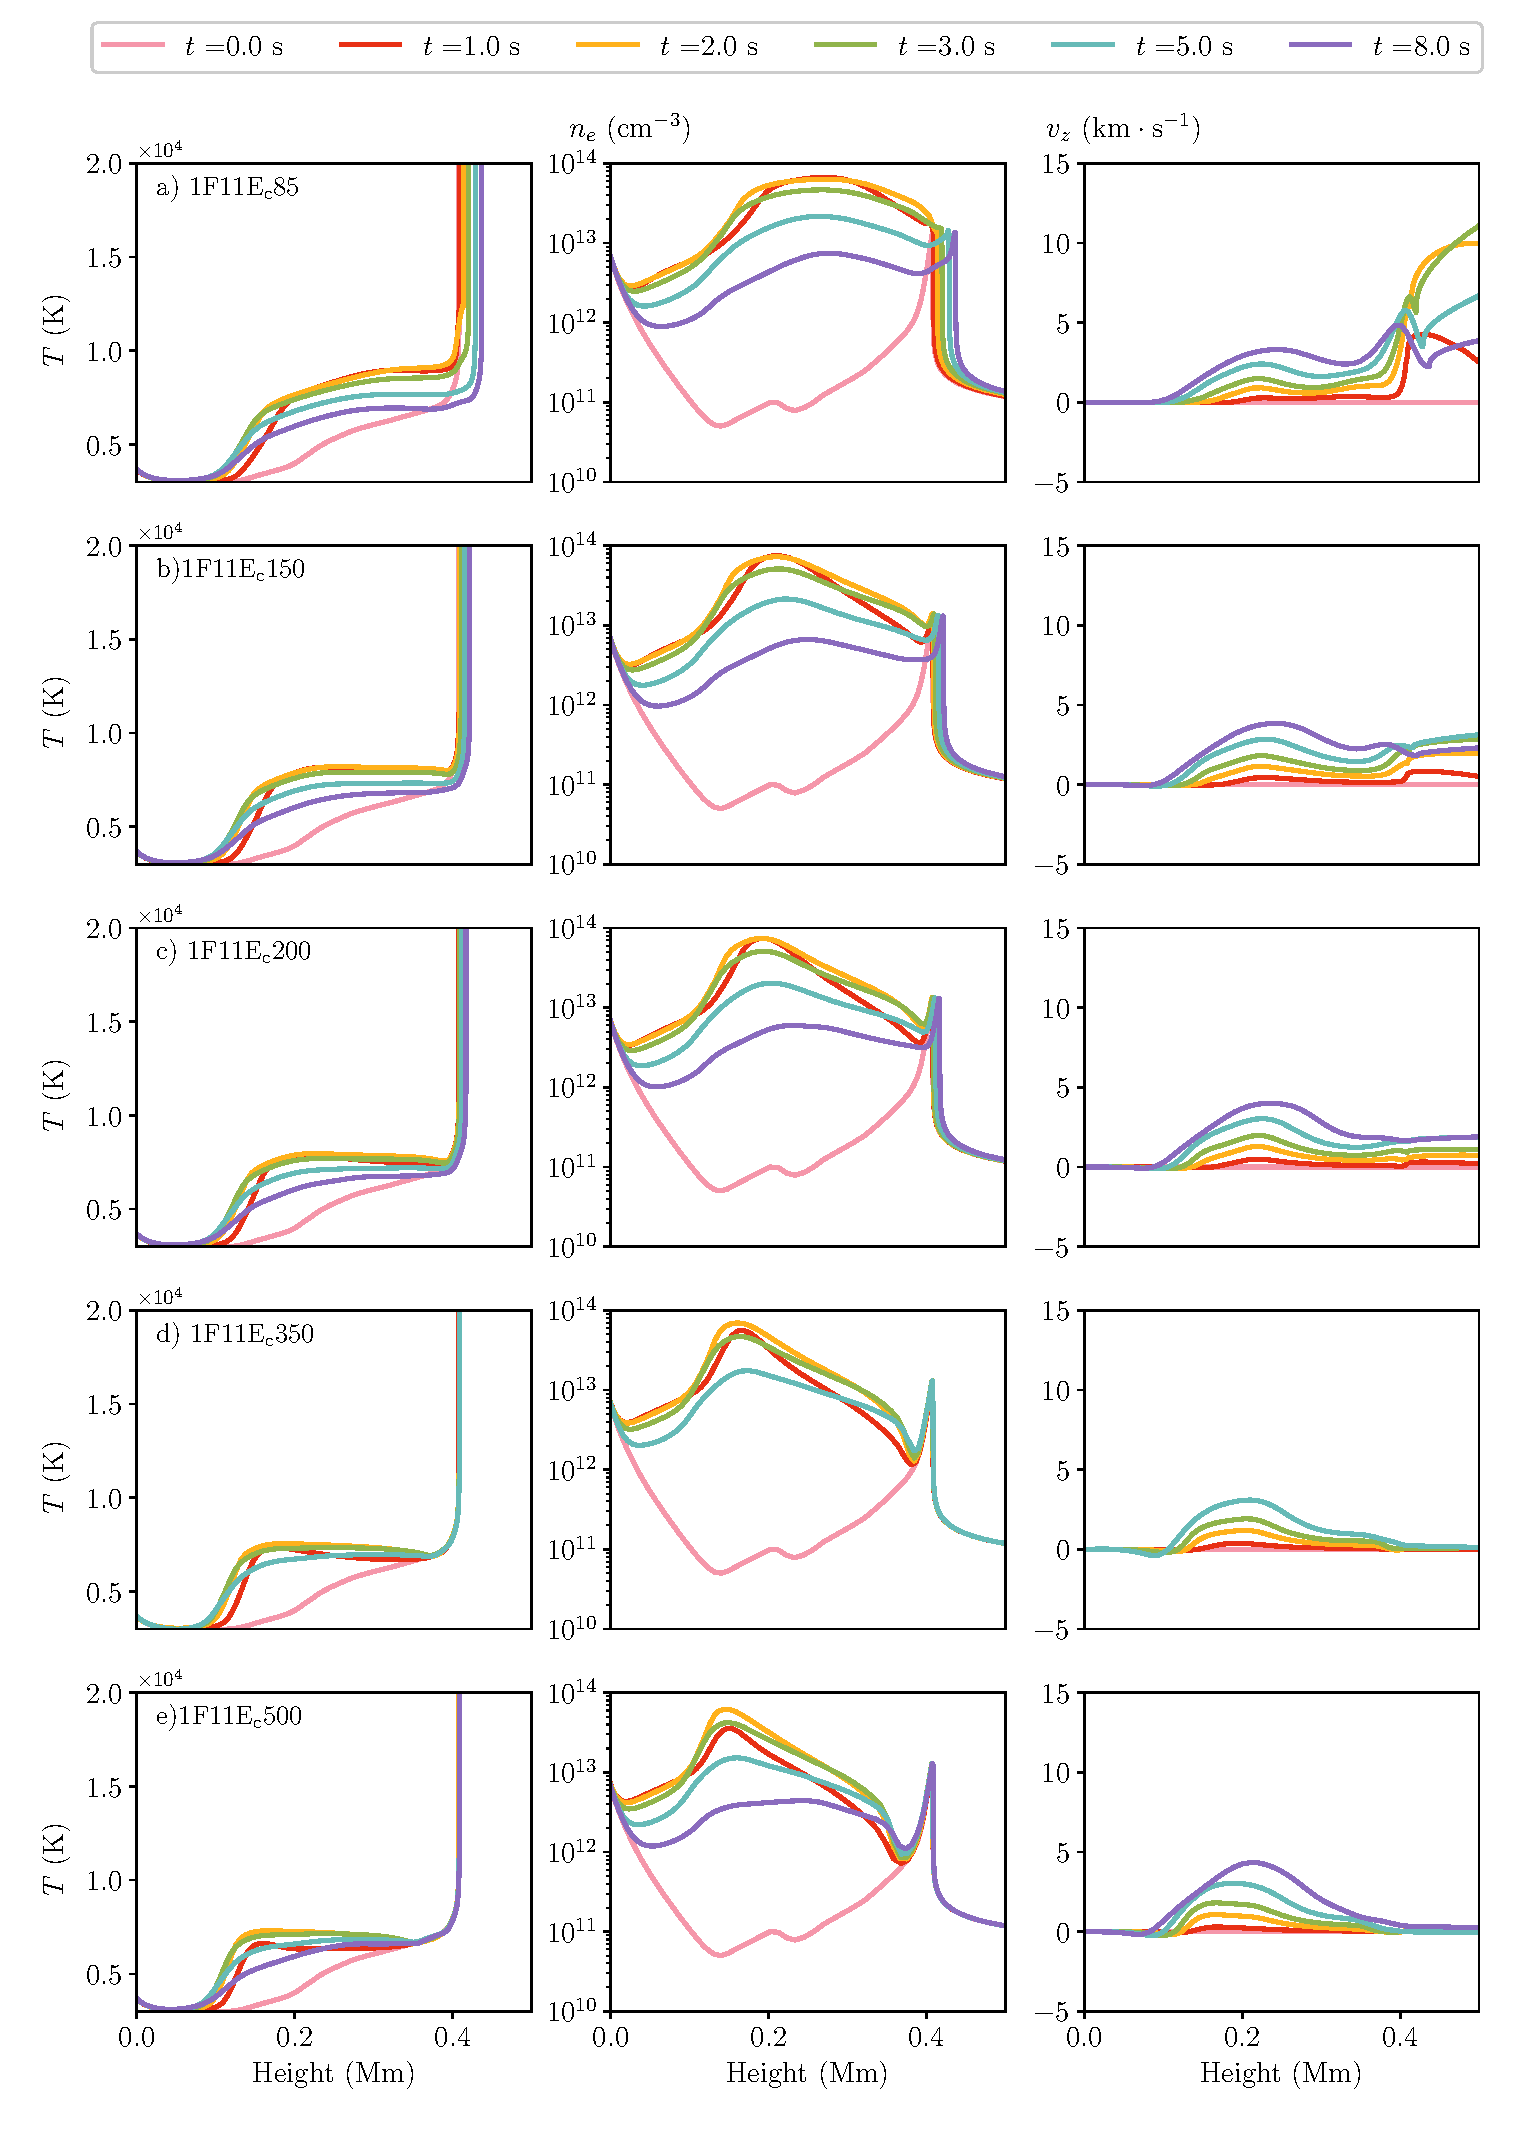
\includegraphics[width=\textwidth]{figs/dMe_atoms_1}
	\caption{各1F11模型中一些特征时刻温度$T$,电子密度$n_e$,一维速度$v_z$随高度分布图。}
	\label{fig:4.1}
\end{figure}

对1F12模型而言,更大的能流输入能够产生更加动态的低层大气。总的来说相比于1F11模型,低层大气能够被加热到更高的温度$\sim 9\times 10^{3}$ K,且能够产生更高的电子密度,接近$10^{15}\ \mathrm{cm^{-3}}$。在$E_c = 85,\ 150 ,\ 200$ KeV时还能在星冕中形成较为可观的物质上流,并且推动过渡区位置上移。

对于高截止能量$E_c$的情况,更低位置的加热使其倾向于产生更低位置的温度极值,且高色球和过渡区基本没有明显的温度、电子密度变化。而对低截止能量$E_c$,仍有部分能量被释放在高色球,使得高色球的温度和电子密度有较大程度的上升,其中温度甚至能够一度上升$10^4$ K达到$2\times 10^4$ K。

\begin{figure}
	\centering
	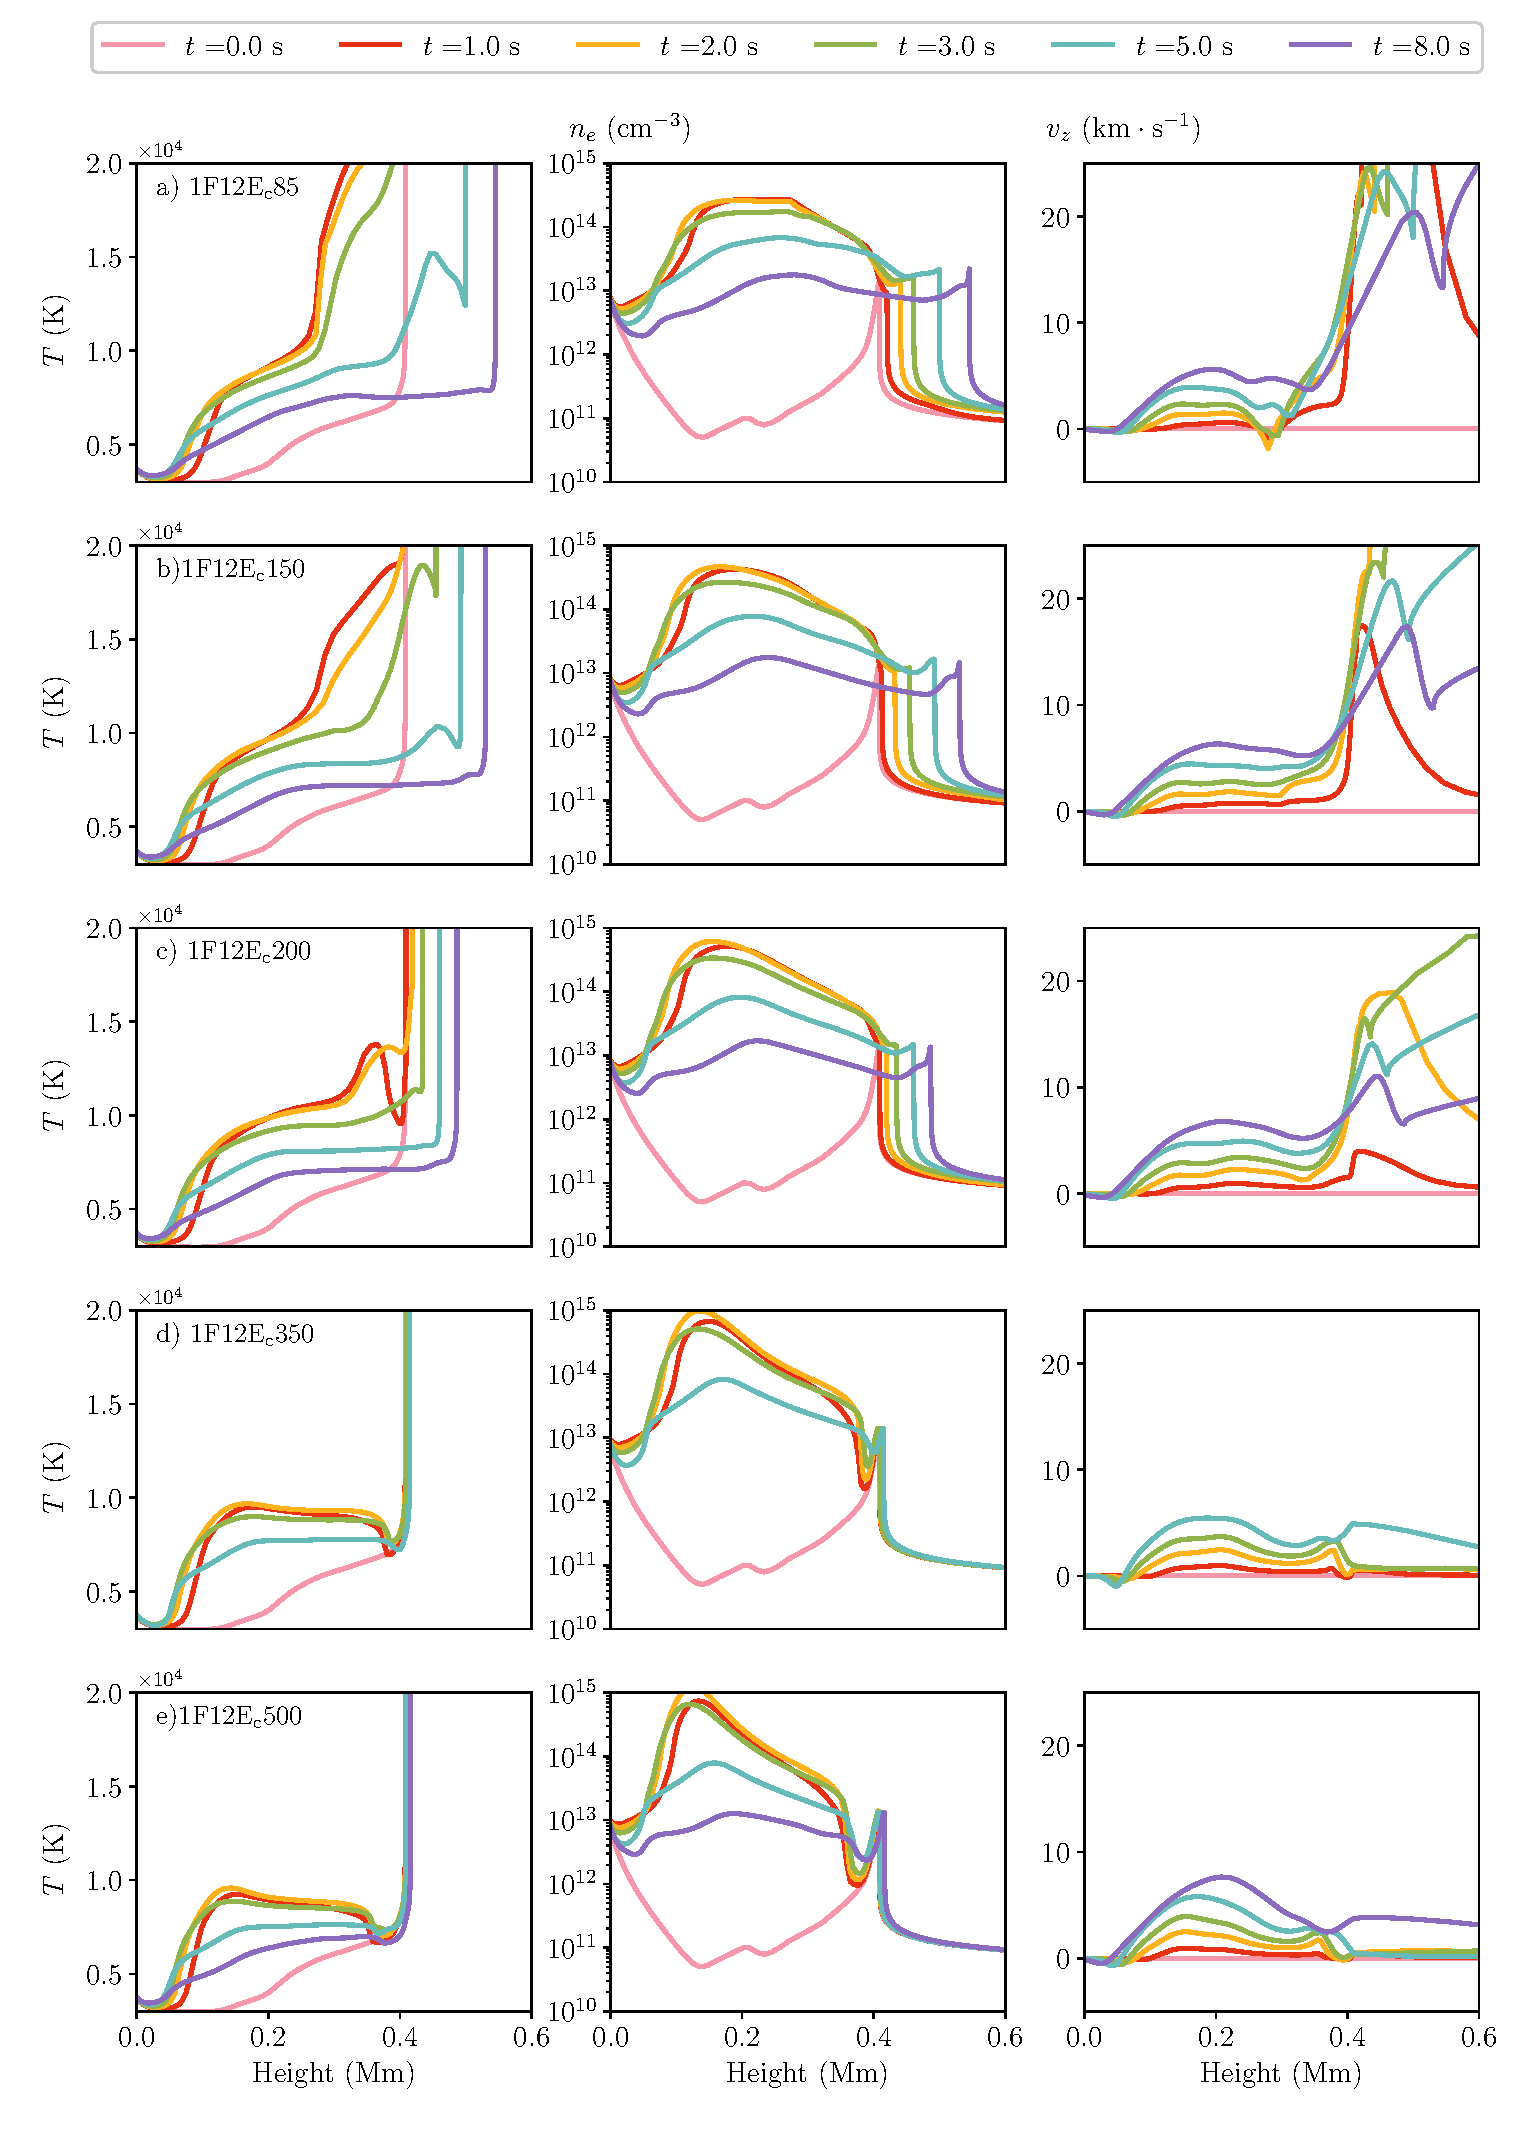
\includegraphics[width=\textwidth]{figs/dMe_atoms_2}
	\caption{各1F12模型中一些特征时刻温度$T$,电子密度$n_e$,一维速度$v_z$随高度分布图。}
	\label{fig:4.2}
\end{figure}

1F13模型相比之前的1F11和1F12模型注入了更大的能流,因此即使是高截止能量下,高色球仍有相当一部分被从低于$10^4$ K的温度加热到$2\times10^4$ K以上。整个中低色球在爆发相的平均温度大约为$\sim 1.5\times 10^4$ K。电子密度$n_e$在爆发相中最高能够达到$10^{16}\ \mathrm{cm^{-3}}$。色球蒸发在色球区域的特征速度大约为$\sim 10-20\ \mathrm{km \  s^{-1}}$。同样高截止能量$E_c$伴随着更低大气中的温度上升,在500 KeV中甚至能在0.1 Mm上达到$2\times 10^4$ K。除了$E_c = 85$ KeV的情况,其他大气中的过渡区伴随着色球蒸发有相对上升。在$E_c = 85$ KeV时色球蒸发的速度上流主要在过渡区以上。

\begin{figure}
	\centering
	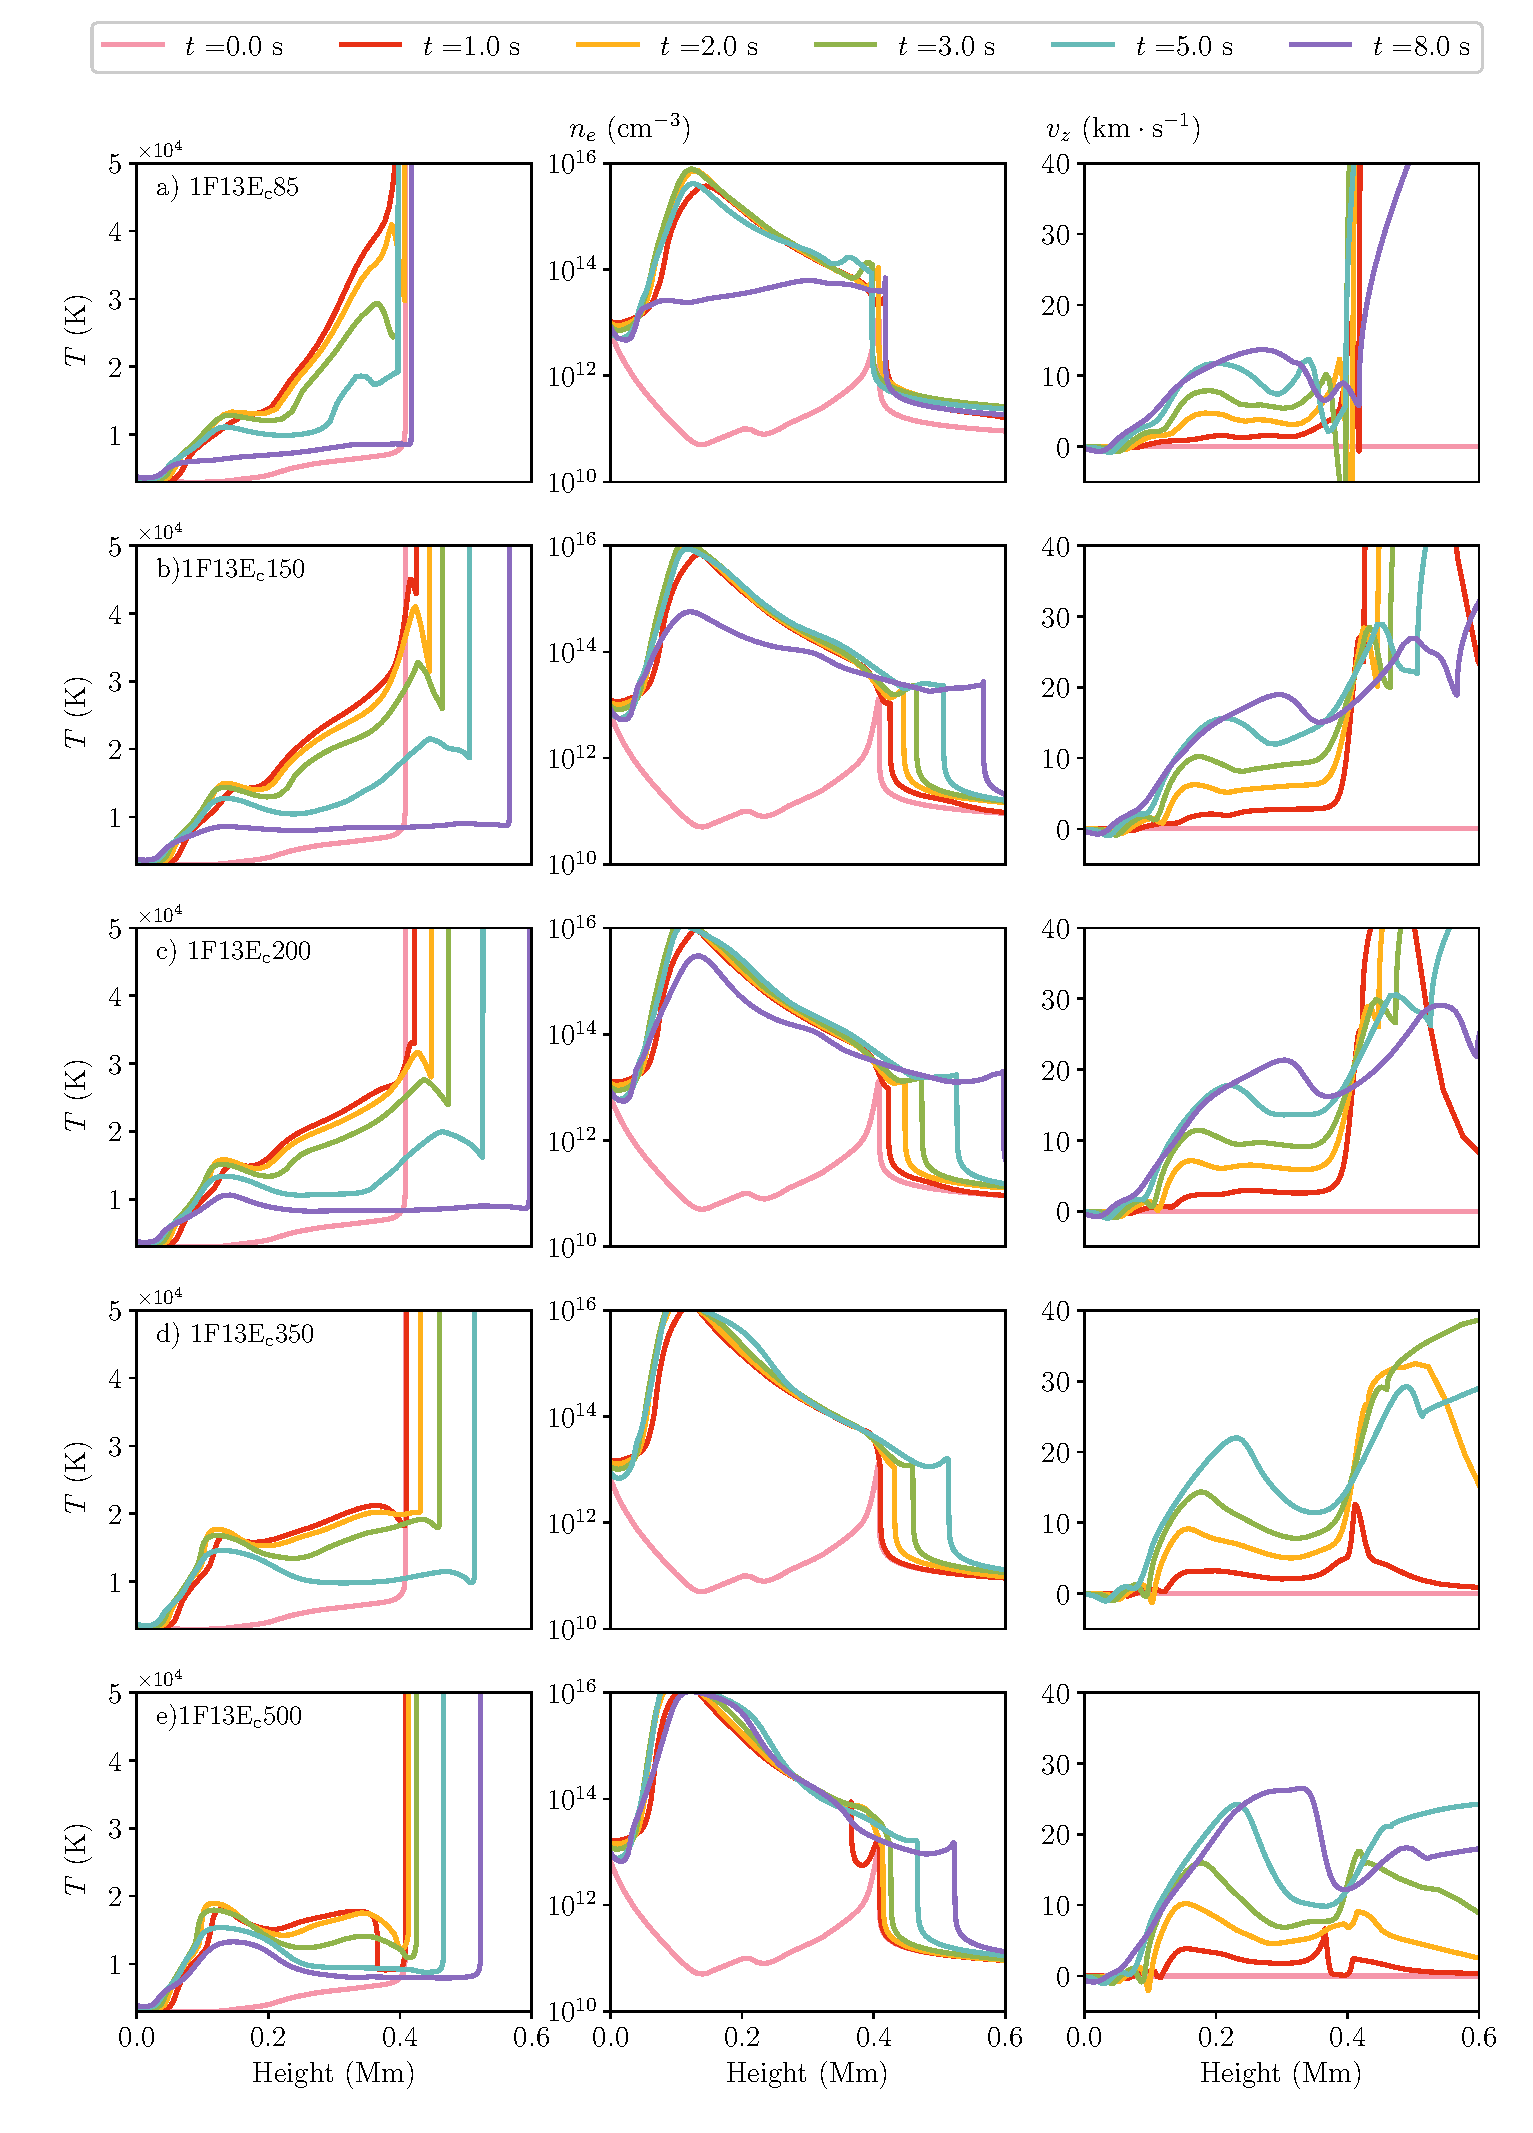
\includegraphics[width=\textwidth]{figs/dMe_atoms_3}
	\caption{各1F13模型中一些特征时刻温度$T$,电子密度$n_e$,一维速度$v_z$随高度分布图。}
	\label{fig:4.3}
\end{figure}

\section{谱线演化特征}\label{sec:4.3}
在这一部分我们将讨论各个模型中的Mg \textsc{ii}谱线演化过程。由于不同非热电子加热大气不同,Mg \textsc{ii}谱线对其也会产生不同的响应。图~\ref{fig:4.4}展示了各个模型中的所有时刻的Mg \textsc{ii} h谱线内总辐射流量随着时间的演化。图~\ref{fig:4.5}展示了~\ref{sec:4.2}节中研究的各个特征时刻的Mg \textsc{ii} h净辐射流量(已经减去初始宁静大气的辐射流量)。可以看到由于整个谱线轮廓较广的形成范围,Mg \textsc{ii} h谱线轮廓事实上包含了两个重要的组成部分,一是线心部分形成于高色球的辐射,和来自于低色球的线翼辐射。因此整个Mg \textsc{ii} h线轮廓形状同时和高低色球两部分的大气参数有着密切联系。

在1F11模型中,除了$E_c=85$ KeV的情况,其他较高截止能量的情况下高色球大气几乎没有变化,因此线心部分的谱线轮廓几乎不发生变化。但是由于低层大气的加热,周围连续谱会有比较强的增强,主要来自于Balmer连续谱的贡献。此外,在部分截止能量$E_c$并不是太大的模拟中,电子密度的高峰并不位于非常深的大气中,而是接近于Mg \textsc{ii} h线翼和线心的形成位置,此时Stark致宽在远线翼位置会发挥比较重要的作用,非常强烈地增强了远线翼的辐射(如图~\ref{fig:4.4}和图~\ref{fig:4.5}的a, b, c等栏)。而此时线心位置如果没有足够的辐射增强(只有$E_c=85$ KeV时比较明显),整个净谱线轮廓会从发射变为吸收(但是真正的谱线轮廓还是发射线)。

在1F12模型中,由于能流有了相对增强,在$E_c=85,\ 150$和200 KeV模拟中基本都可以看到Mg \textsc{ii} h线心辐射的增强。且原来线心反转的谱线出现明显的红翼增强,在某些时刻甚至出现了非线心反转的谱线轮廓($t=2.0$ s等)。而在$E_c$较大时的谱线轮廓和1F11类似,都是连续谱剧烈增强但线心辐射基本没有明显变化,净谱线轮廓看上去像是吸收线。

1F13模型的谱线轮廓和之前的两个模型有较大不同,其一是由于低色球和高光球都被加热,因此整个谱线线翼的连续谱都剧烈增强。而且这些增强并非全部来自于Mg \textsc{ii} h线自身的Stark致宽,还有大量由于自由电子复合过程产生的Balmer连续谱的贡献。由于在高色球Mg \textsc{ii}线线心形成位置形成了较大的速度上流,谱线普遍表现出一定的蓝移特征,且伴随着一定的红翼辐射增强。在$E_c = 350$和500 KeV的模拟中,由于连续谱过于剧烈的增强,再发射也无法抵消吸收,Mg \textsc{ii} h线真的成为了吸收线。由于谱线的不对称性,在部分$E_c = 350$ KeV的谱线中可以看到红翼出现发射,而蓝翼出现吸收的特殊净谱线轮廓。


\begin{figure}
	\centering
	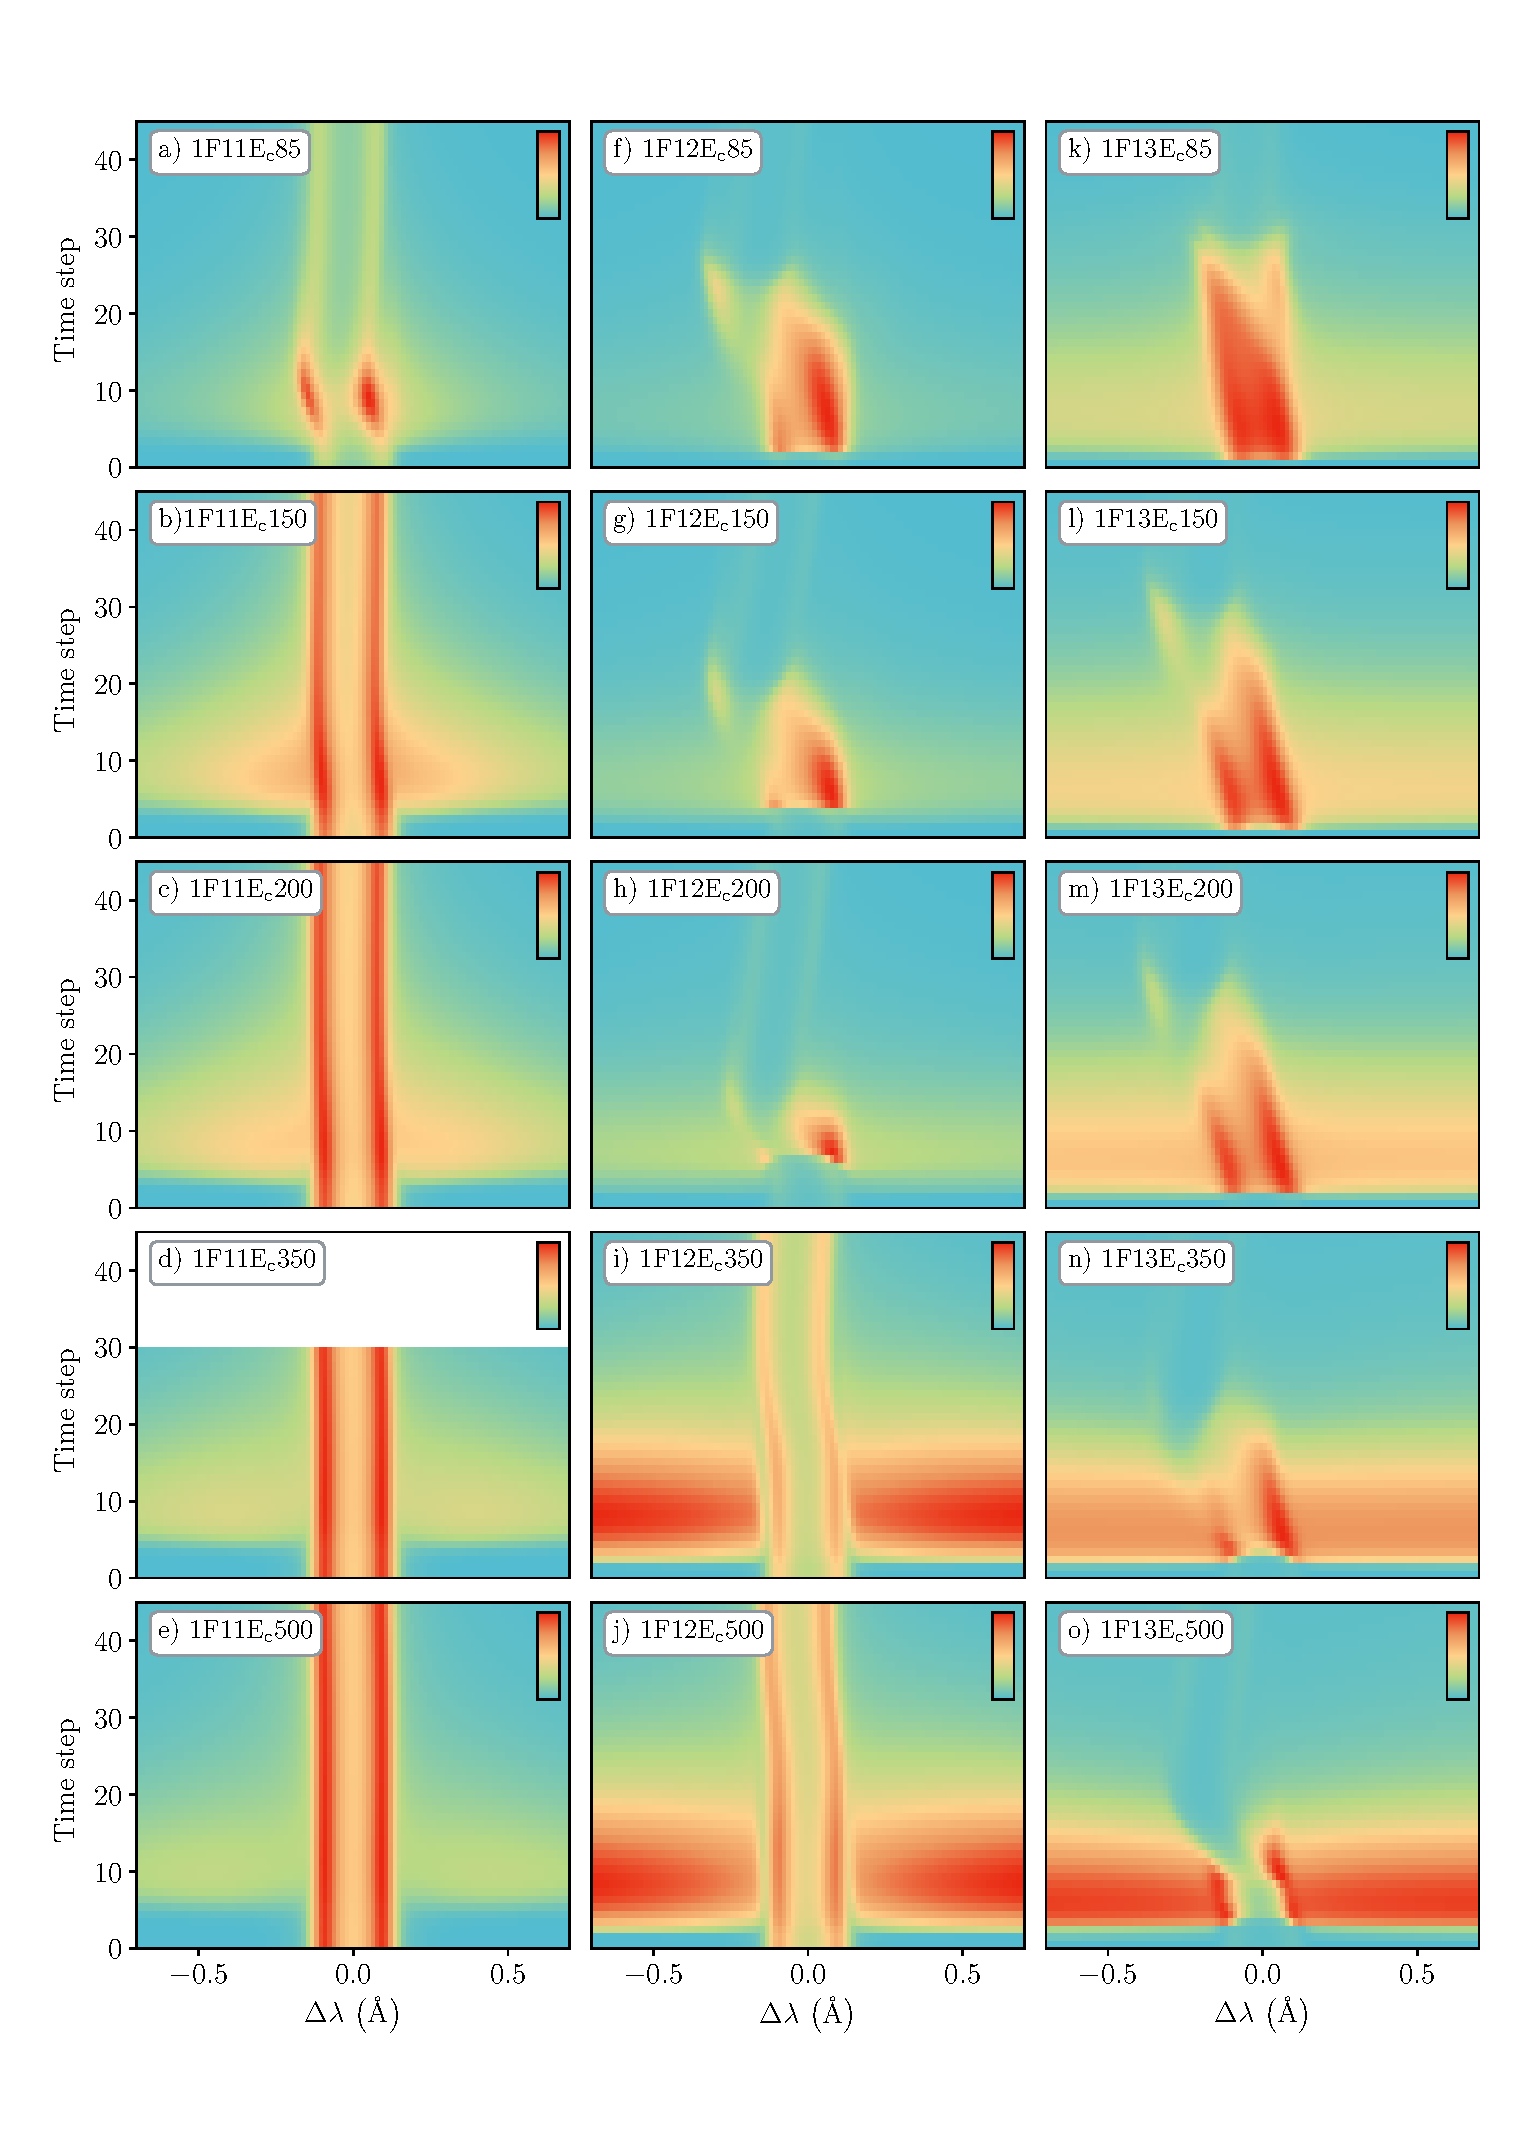
\includegraphics[width=\textwidth]{figs/dMe_MgIIh}
	\caption{Mg \textsc{ii} h线在不同电子束参数的模拟中的谱线流量随时间演化图。横坐标为波长,纵坐标为不同时刻,颜色代表该波长和时刻下的辐射流量。}
	\label{fig:4.4}
\end{figure}

\begin{figure}
	\centering
	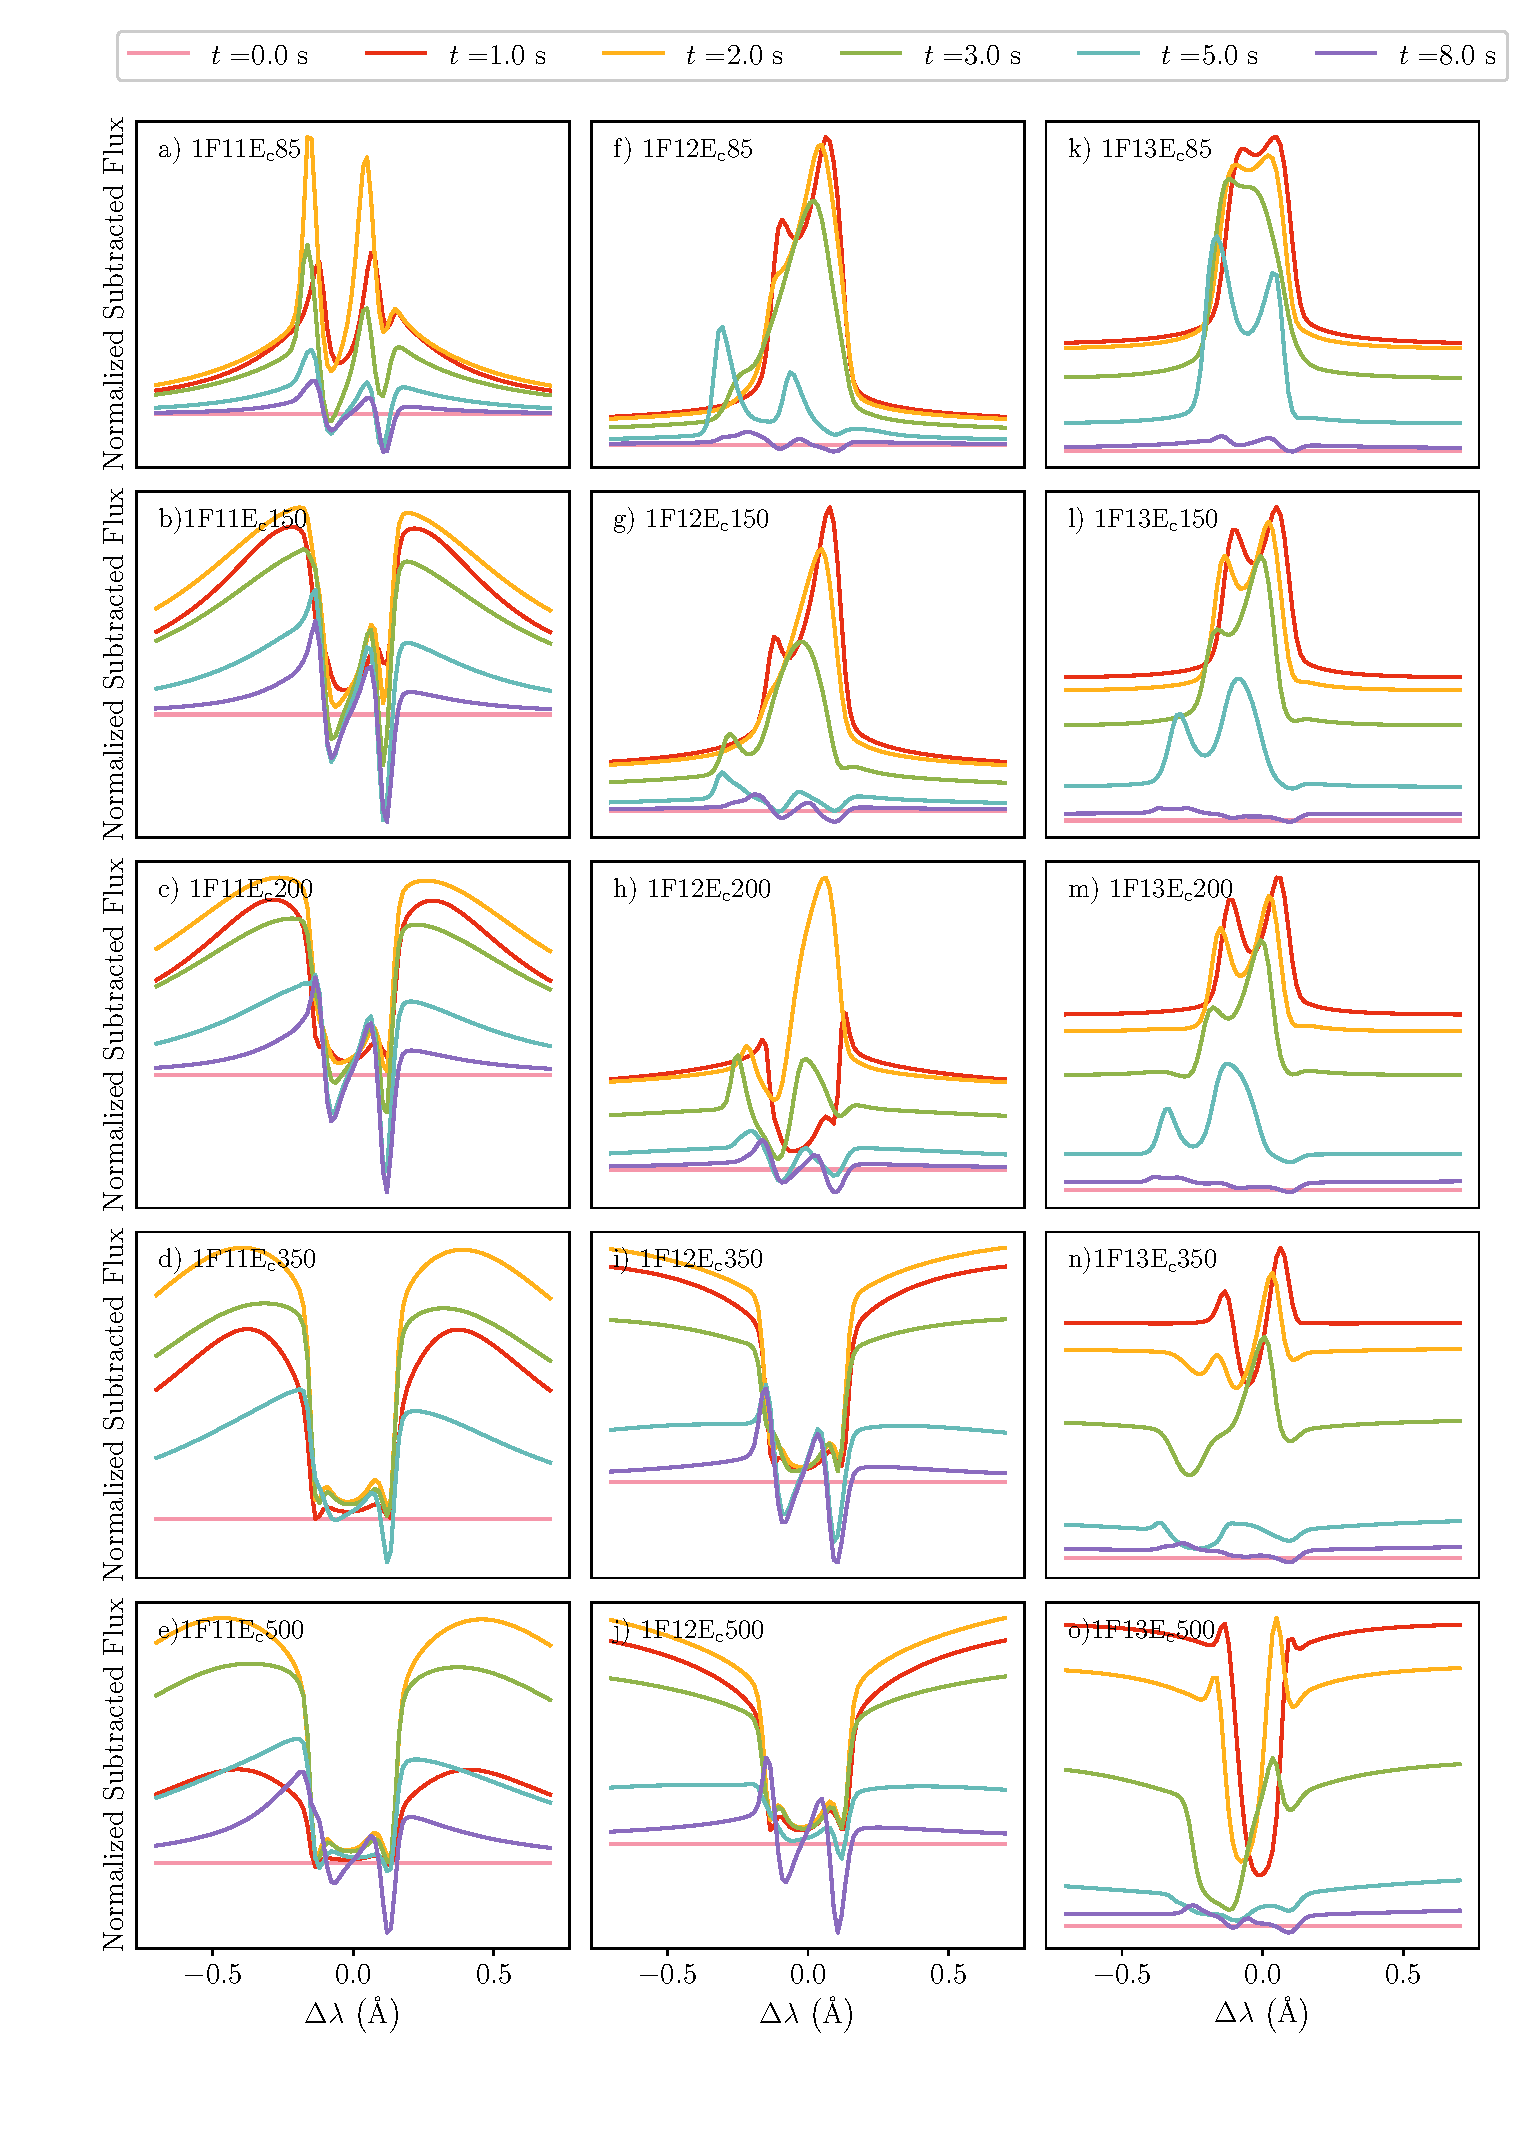
\includegraphics[width=\textwidth]{figs/dMe_MgIIh_spec}
	\caption{Mg \textsc{ii} h线在不同电子束参数的模拟一些特征时刻的谱线轮廓。注意图中展示的是已经减掉宁静初始大气辐射的净辐射流量。}
	\label{fig:4.5}
\end{figure}

\begin{figure}
	\centering
	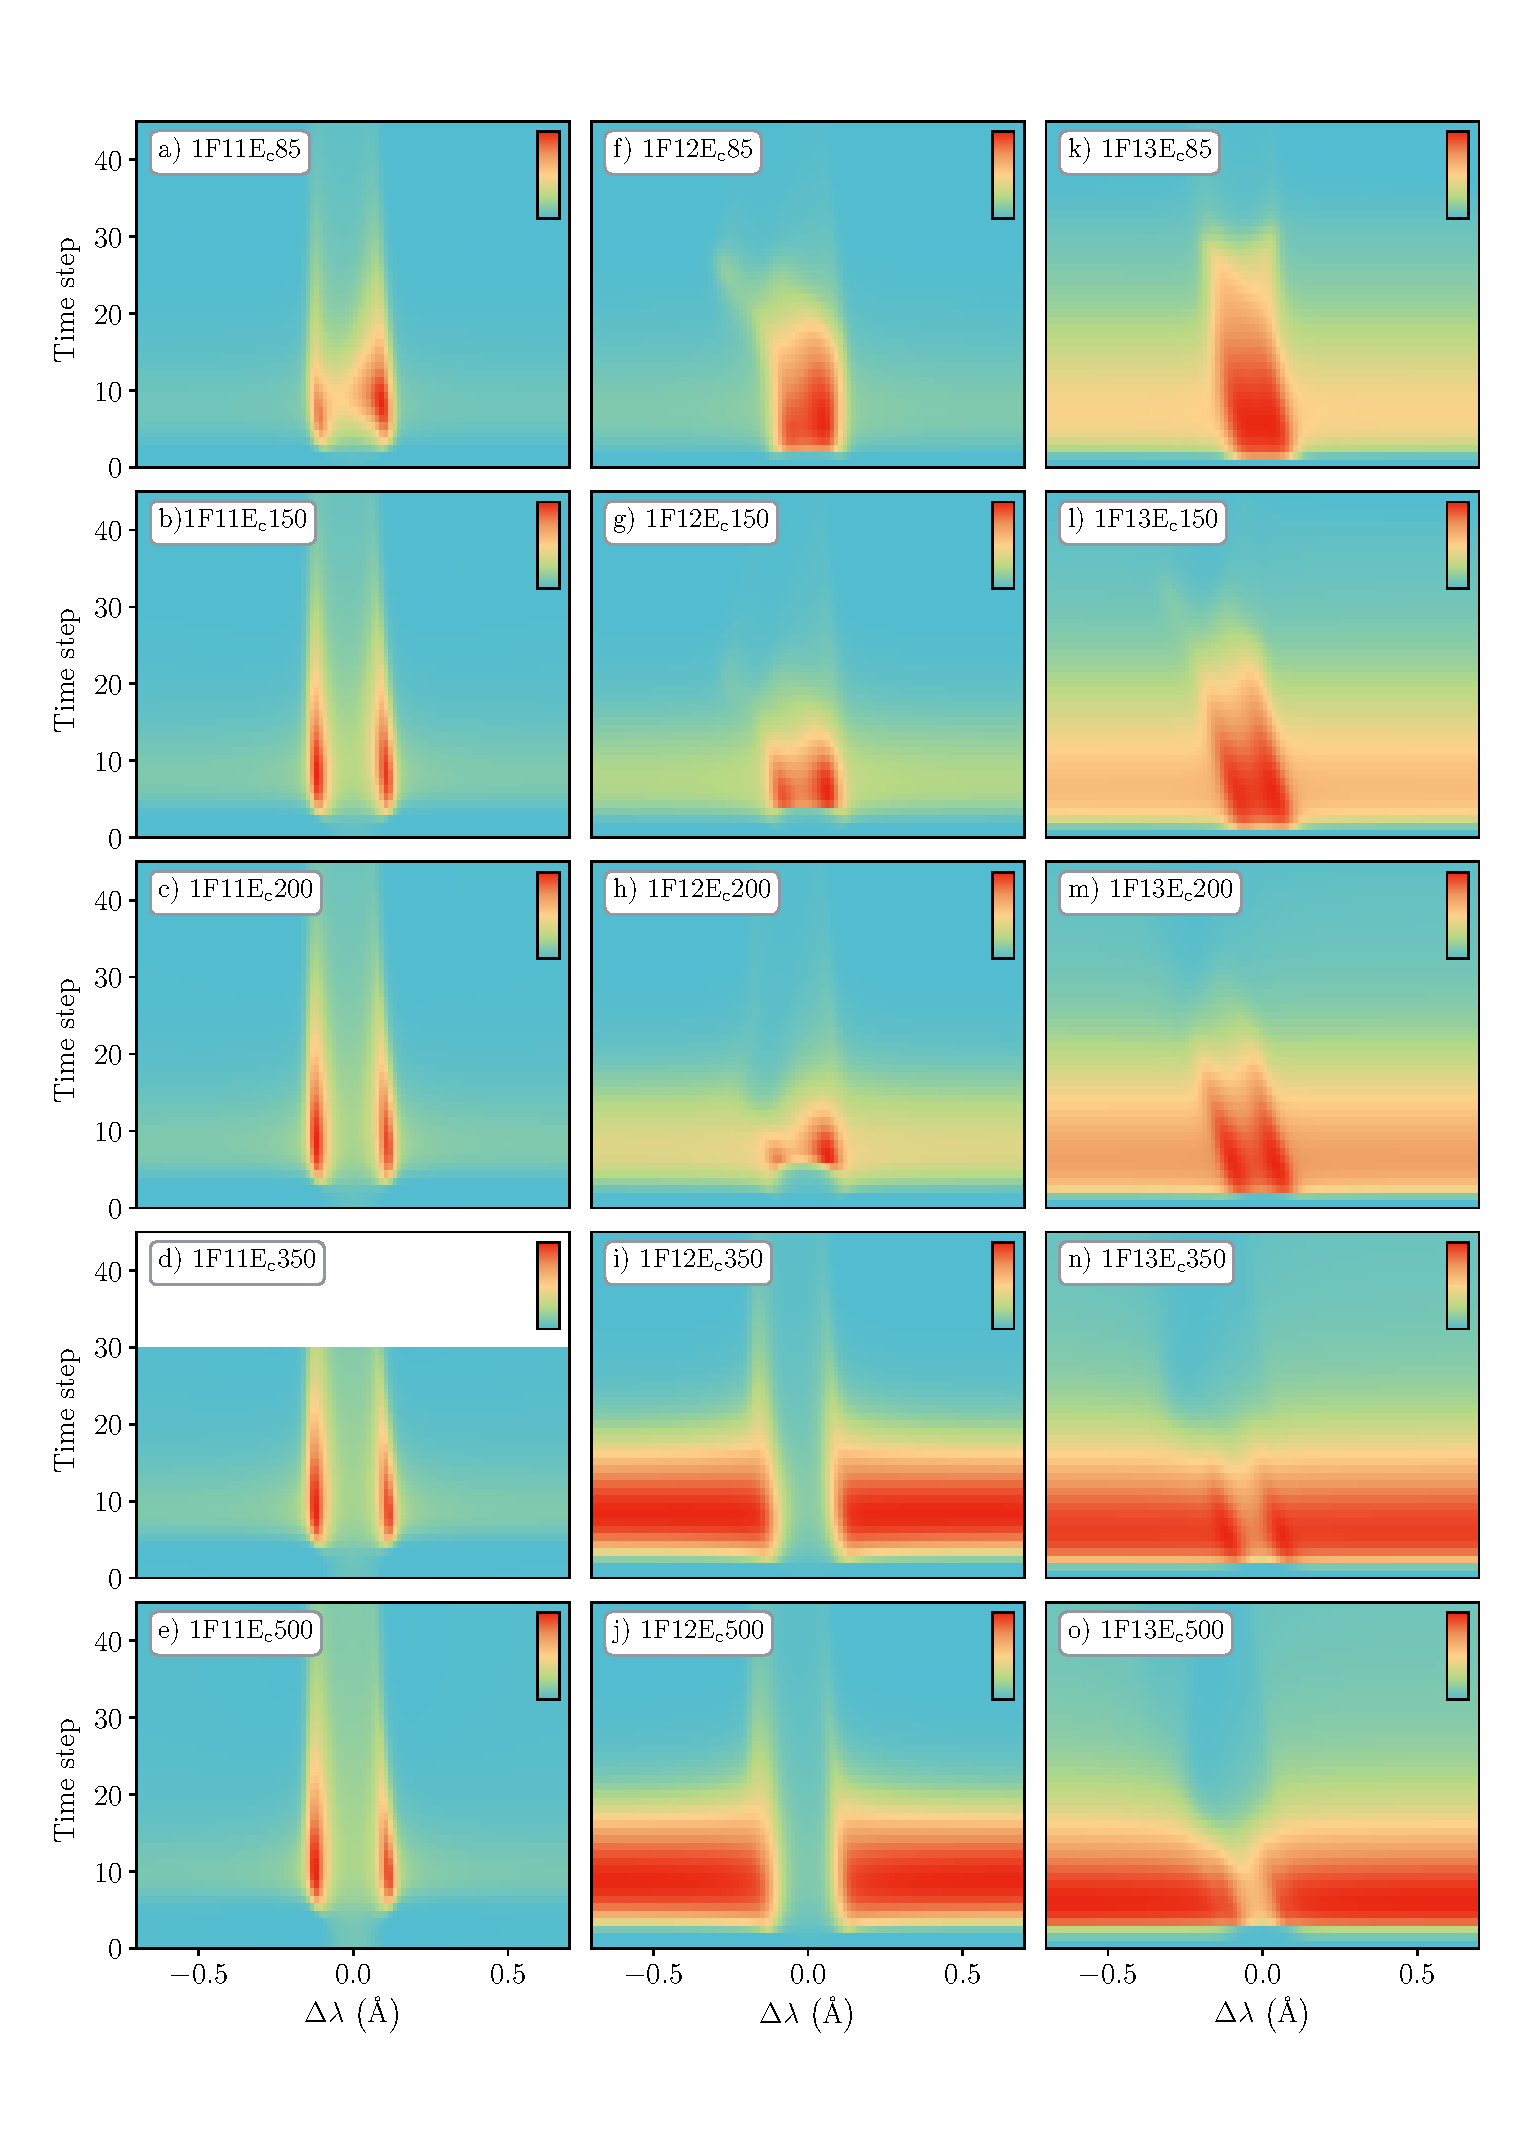
\includegraphics[width=\textwidth]{figs/dMe_MgII_2791}
	\caption{Mg \textsc{ii} 2791 \mbox{\AA}线在不同电子束参数的模拟中的谱线流量随时间演化图。}
	\label{fig:4.6}
\end{figure}

\begin{figure}
	\centering
	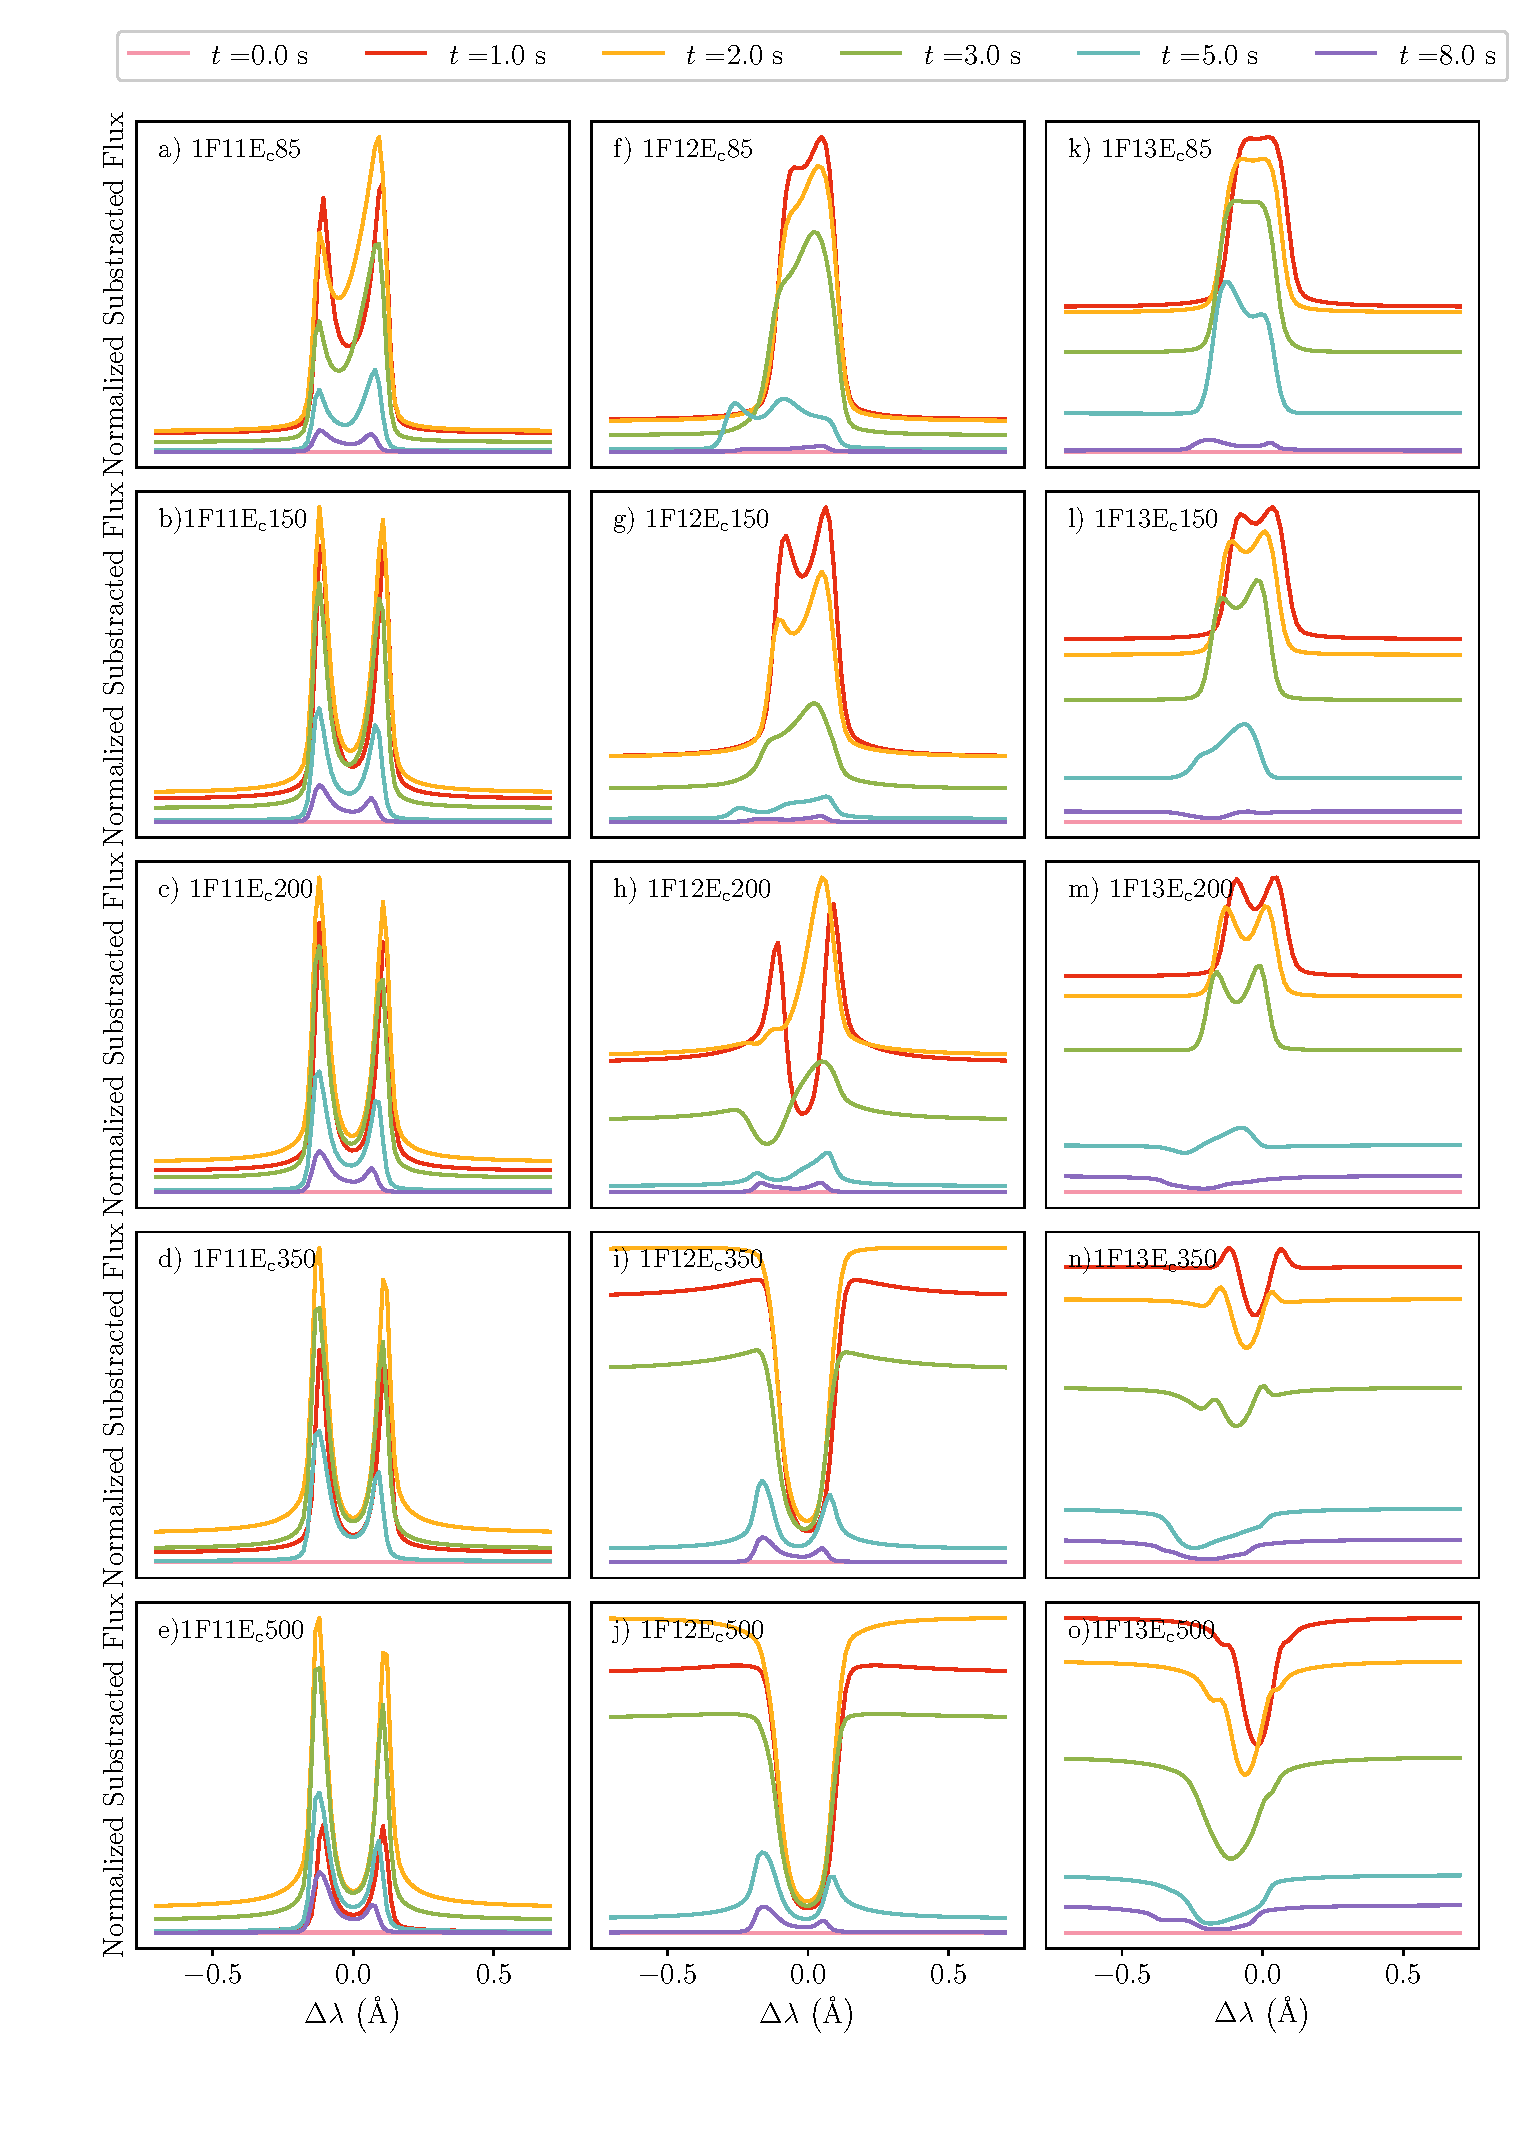
\includegraphics[width=\textwidth]{figs/dMe_MgII2791_spec}
	\caption{Mg \textsc{ii} 2791 \mbox{\AA}线在不同电子束参数的模拟一些特征时刻的谱线轮廓。注意图中展示的是已经减掉宁静初始大气辐射的净辐射流量。}
	\label{fig:4.7}
\end{figure}

和太阳上的Mg \textsc{ii} 2791 \mbox{\AA}有所不同的是,在\ref{sec:4.4}节中我们将会看到Mg \textsc{ii}三重线的线心形成高度事实上是和Mg \textsc{ii} h和k线相当接近的,不同的是Mg \textsc{ii} 三重线的线翼会形成在更深的位置。因此和Mg \textsc{ii} h线类似,三重线的谱线轮廓演化会随高色球和低色球两部分的加热、速度分布不同而表现出不同的轮廓形状。

在1F11模型中,大部分的Mg \textsc{ii} 2791 \mbox{\AA}线的轮廓形状都类似,表现为在线心处没有剧烈增强,但是在靠近线心的两翼有明显增强,而在更远的线翼位置,谱线同样由于Stark致宽而有一定程度的辐射增强。

在1F12和1F13模型中,三重线谱线轮廓变化展现出完全不同的演化特征。在相对较低的截止能量$E_c$时,谱线线心出现的明显的辐射增强,并出现一定程度的红翼增强。在$E_c$较大时,周围连续谱剧烈增强,谱线又重新变为吸收线。




\section{形成高度分析}\label{sec:4.4}

\begin{figure}
	\centering
	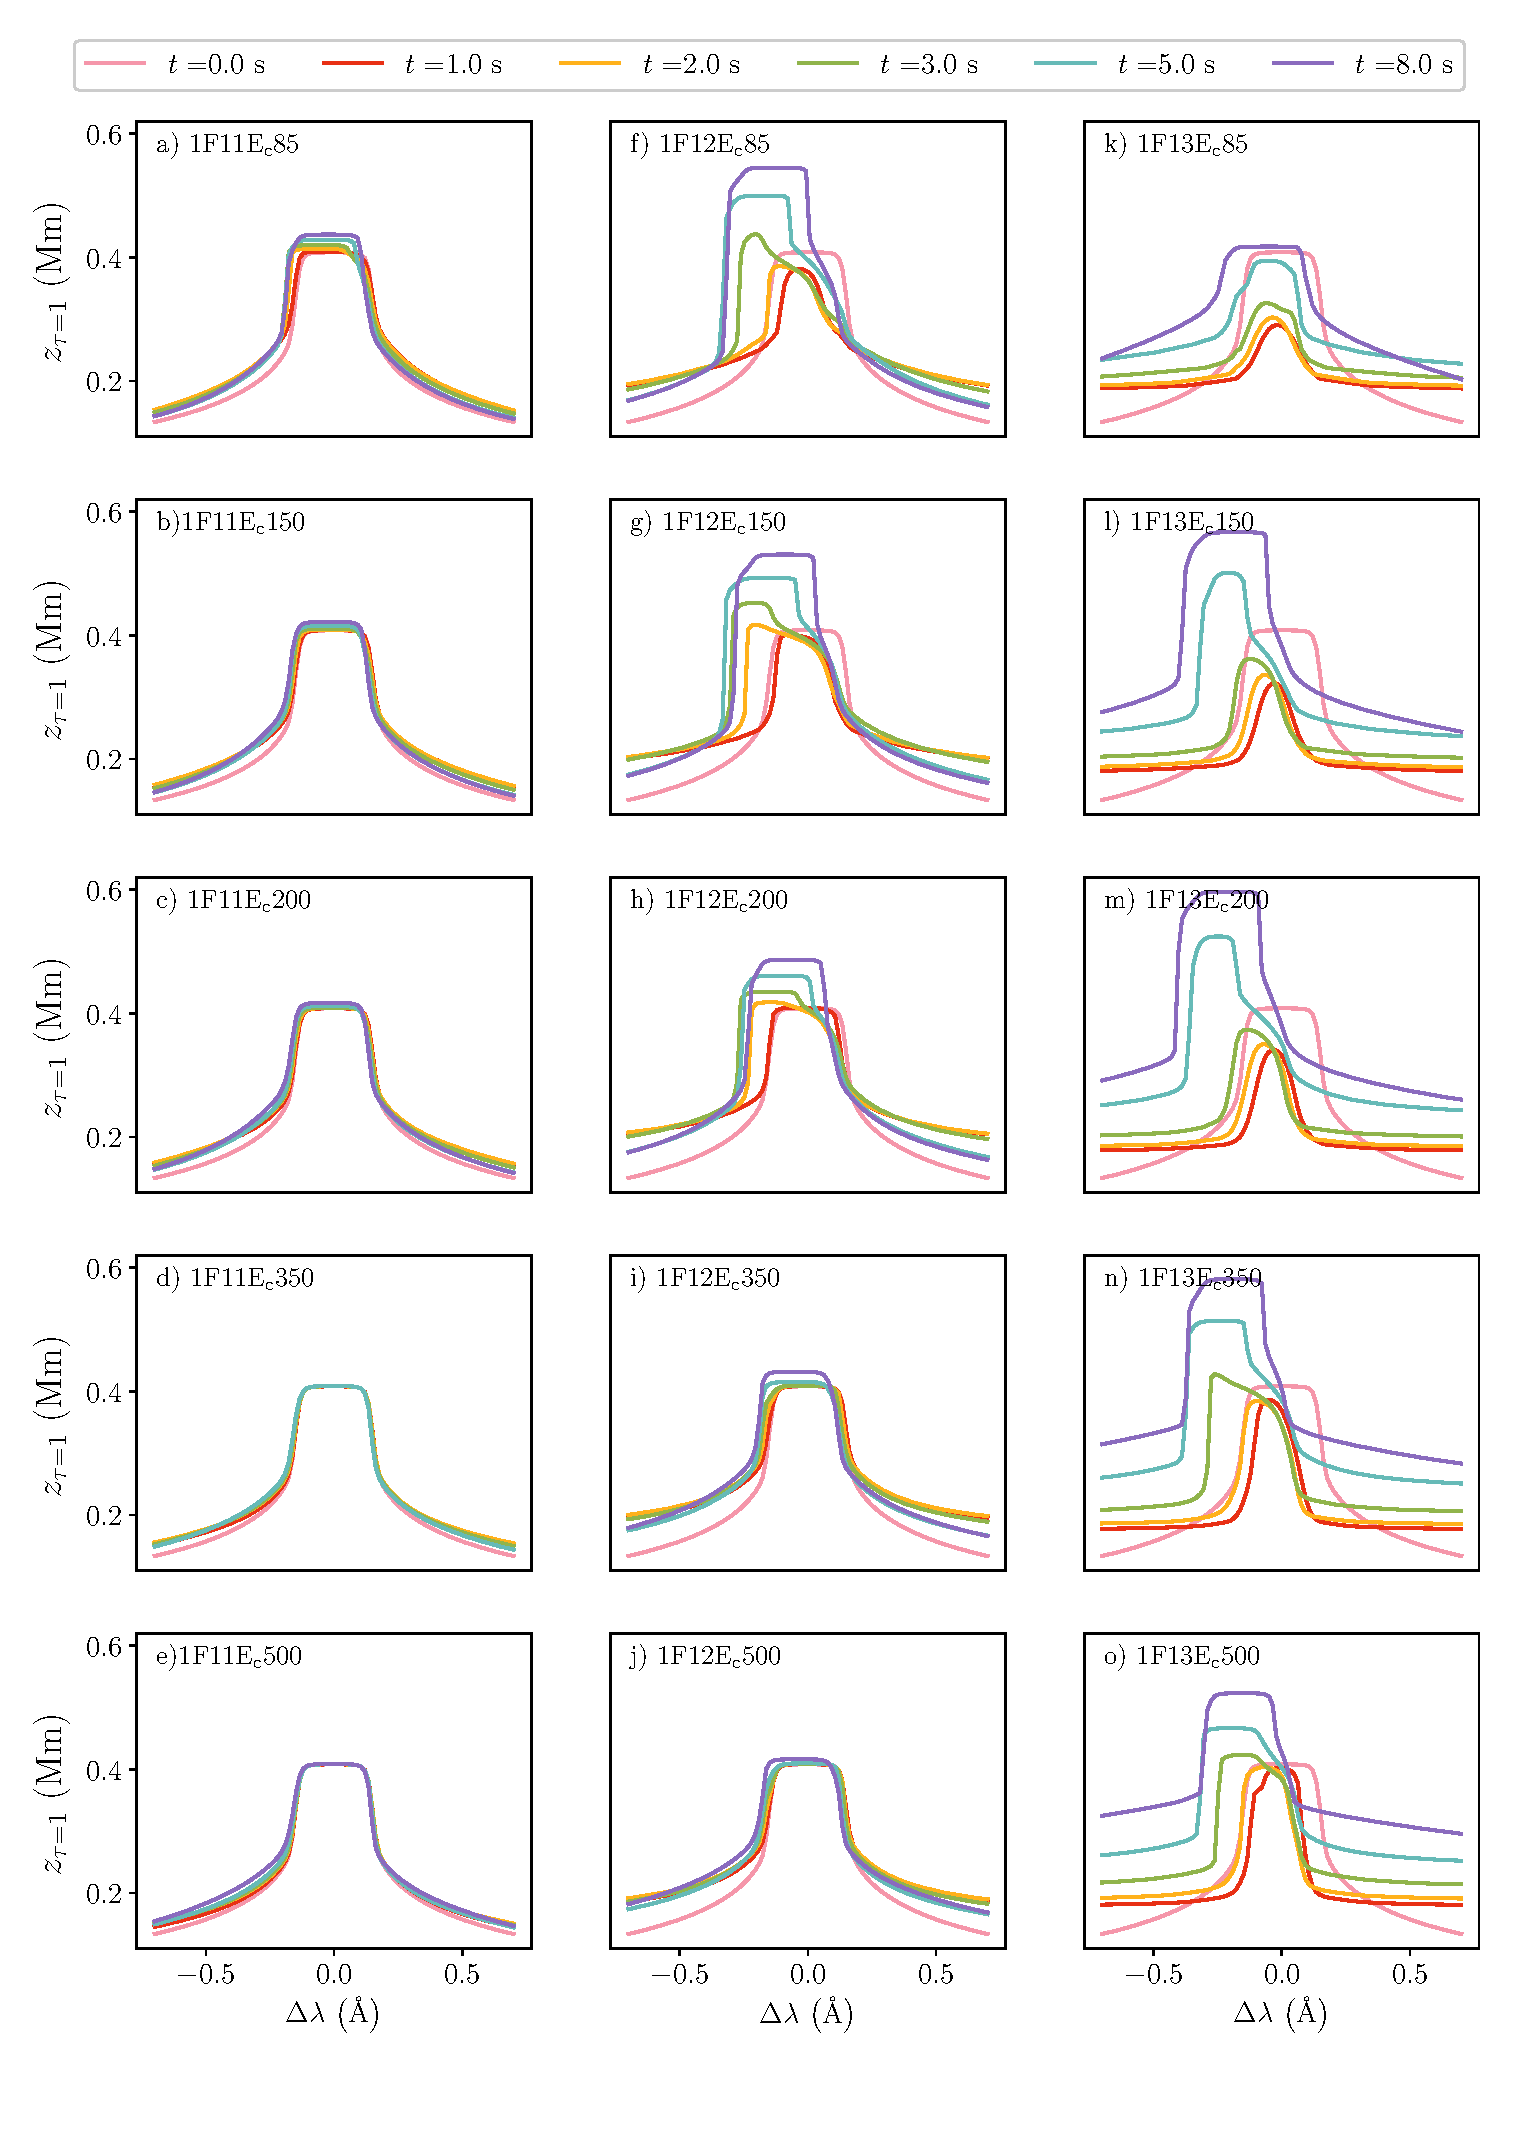
\includegraphics[width=\textwidth]{figs/dMe_MgIIh_tau1}
	\caption{Mg \textsc{ii} h线在不同电子束参数加热情况下谱线范围内的光学深度$\tau = 1$的高度$z_{\tau=1}$随时间演化图。}
	\label{fig:4.8}
\end{figure}

\begin{figure}
	\centering
	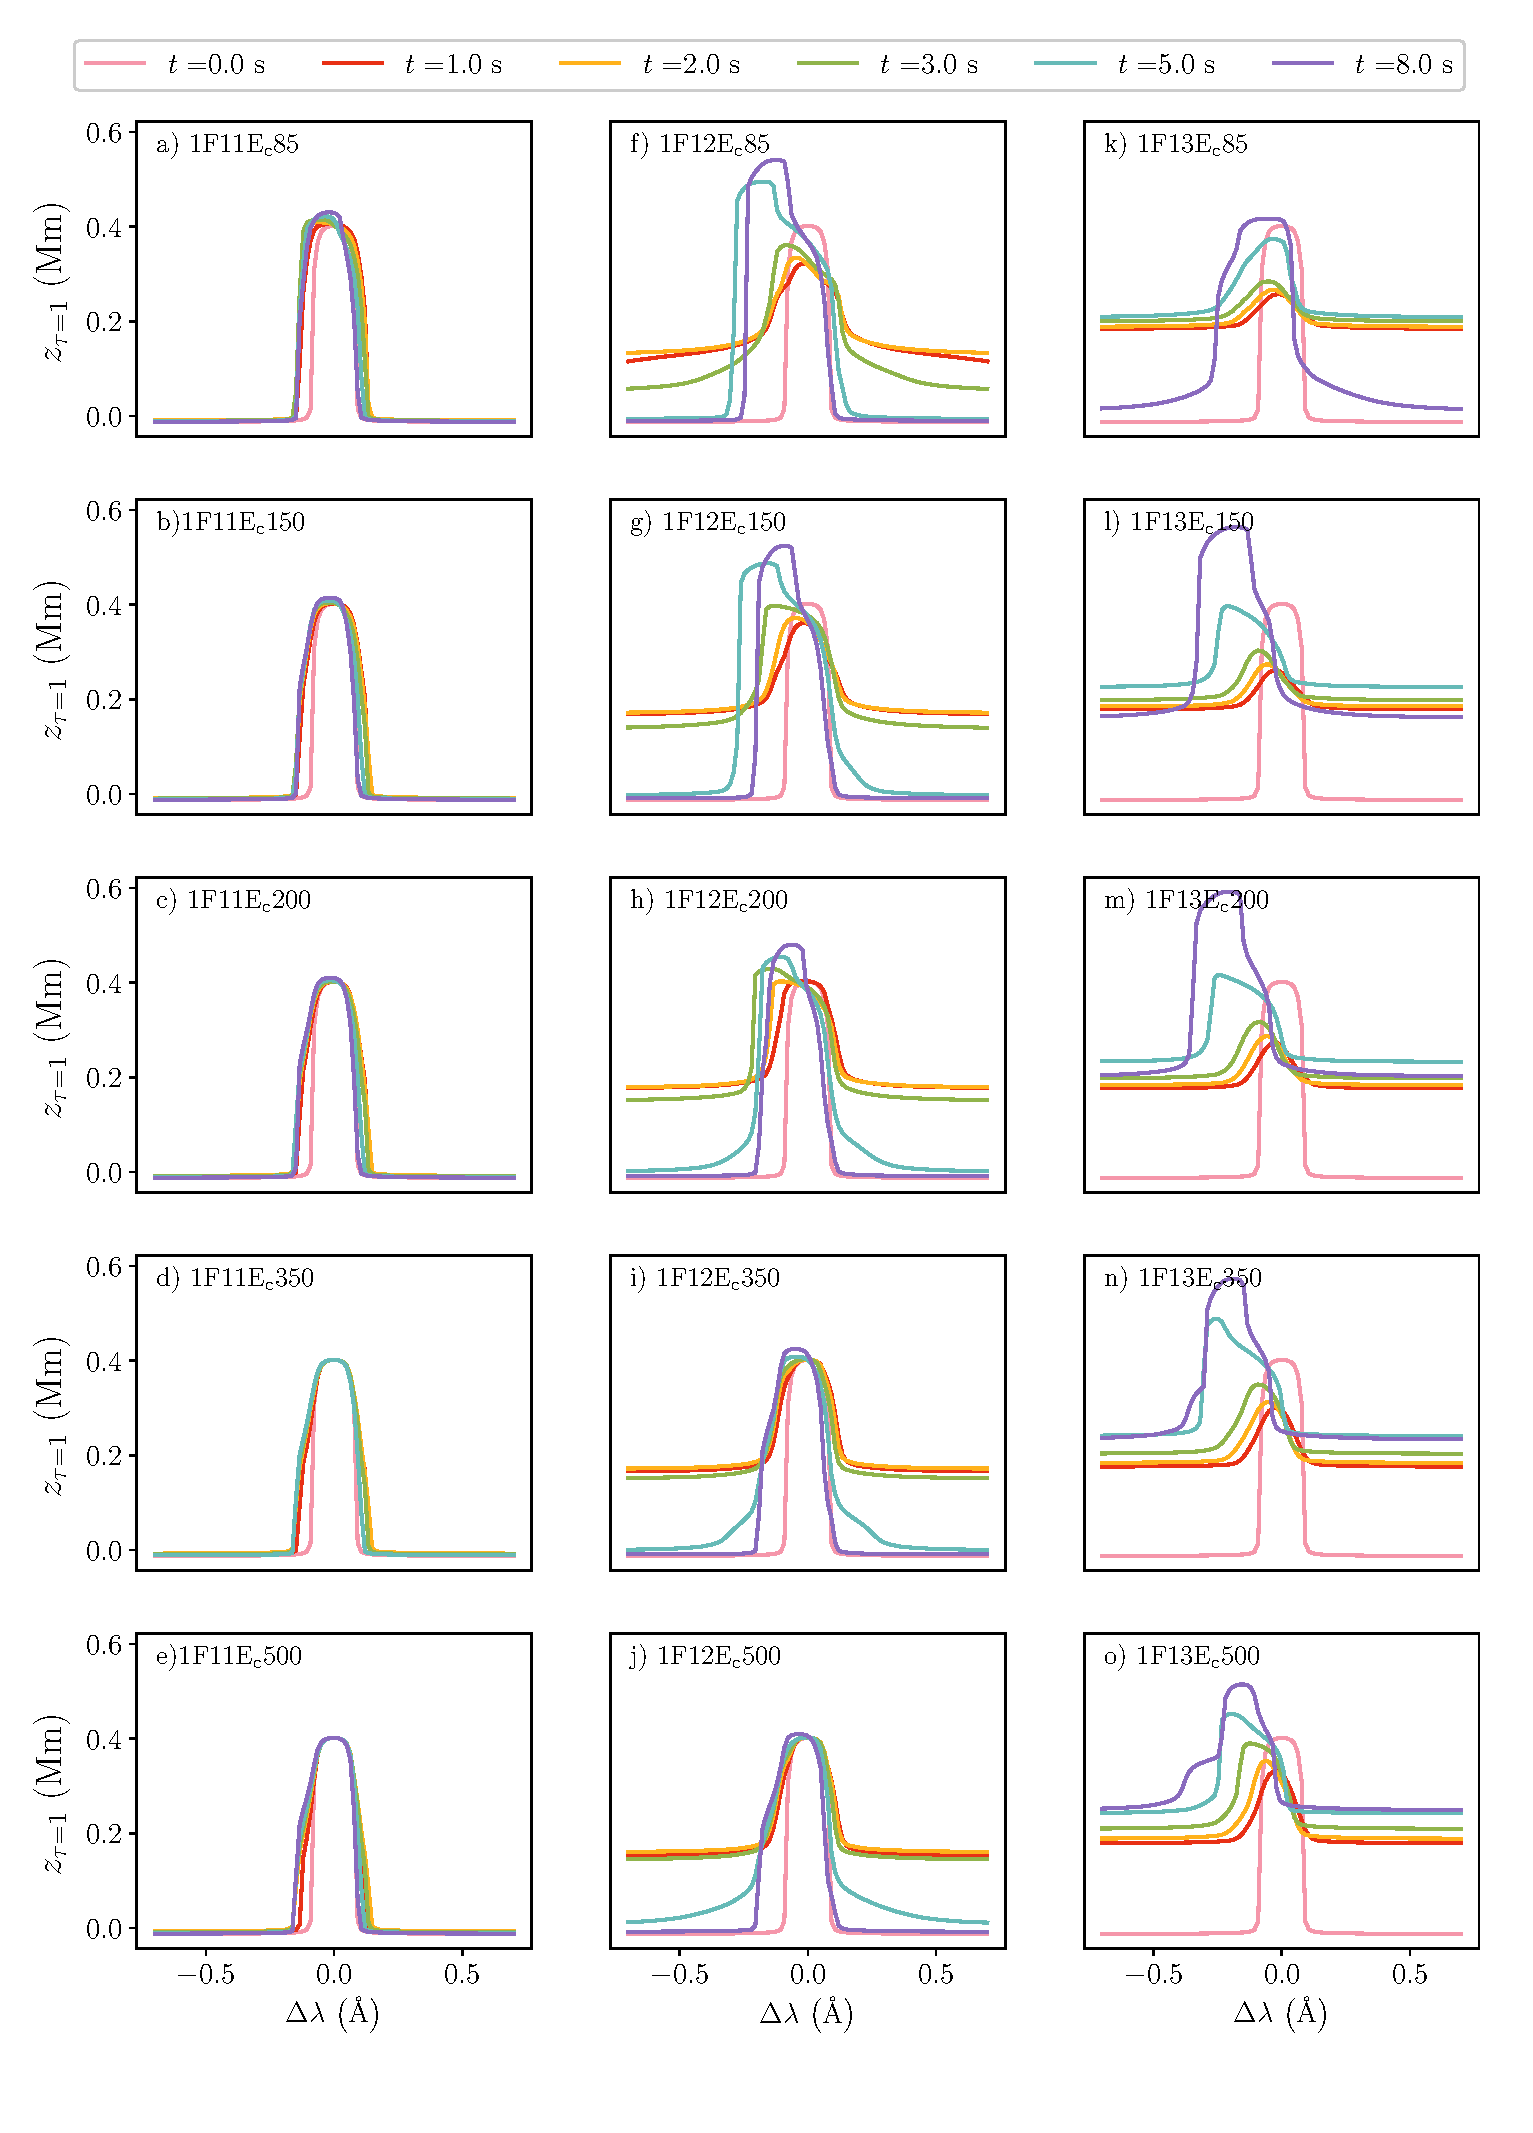
\includegraphics[width=\textwidth]{figs/dMe_MgII2791_tau1}
	\caption{Mg \textsc{ii} 2791 \mbox{\AA}线在不同电子束参数加热情况下谱线范围内的光学深度$\tau = 1$的高度$z_{\tau=1}$随时间演化图。}
	\label{fig:4.9}
\end{figure}

我们在这一节中主要依靠光学深度$\tau_\nu = 1$的对应高度$z_{\tau = 1}$来确定光学厚的Mg \textsc{ii}谱线轮廓在M矮星大气中的形成高度。结合\ref{sec:4.2}中的大气演化参数,对\ref{sec:4.3}节中的一些特征的谱线轮廓的形成做一个简单的解释。图~\ref{fig:4.8}中展示了Mg \textsc{ii} h线轮廓内$\tau_\nu = 1$的高度在之前的特征时刻随波长的分布。一个和太阳大气的明显区别就是在宁静的M矮星大气中,我们发现Mg \textsc{ii} h和k线的线心$\tau = 1$高度和三重线的$\tau = 1$高度比较接近($\sim 0.4 $ Mm)。但三重线的线翼形成在非常低的高度上($\sim 0$ Mm),而Mg \textsc{ii} h和k线线翼形成在相对较高的位置上($\sim 0.2$ Mm)。

在1F11的模型中,所有的Mg \textsc{ii} h和2791 \mbox{\AA}线的形成高度基本没有发生变化。Mg \textsc{ii} h的线翼形成在电子密度约为$10^{14}\ \mathrm{cm^{-3}}$的区域内,因此谱线的Stark致宽非常明显。由于线心形成位置的大气参数几乎没有变化(除了$E_c = 85$ KeV),因此线心强度没有明显变化。而Mg \textsc{ii} 2791 \mbox{\AA}在线心两旁的增强则是来自于低层大气的加热导致的这些频率位置的$\tau = 1$高度上升而靠近线心形成位置,因此这部分的辐射强度因为形成高度温度较高,而明显增强。

在1F12的模型中,Mg \textsc{ii}线和2791三重线的$\tau = 1$层随时间演化和对模型的依赖关系都比较相近,形成的谱线轮廓也有相似之处。相对较小截止能量$E_c$时线心辐射增强而形成的发射线主要来自于上色球部分的加热,其红翼不对称性主要来自于上流物质引起的蓝翼$\tau = 1$层的高度进一步上升,因此蓝翼相对辐射较小,出现红翼不对称性。而在高截止能量的情况下,线心附近的$\tau =1$层并不变化,表现为线心辐射强度基本不变。所有的1F12模型的谱线线翼的形成高度均有所上升,特别是在高截止能量$E_c$的模型中,其线翼形成高度基本和低色球的温度极值区域相重合,因此表现在光谱上是连续谱由于自由电子复合产生的Balmer连续谱辐射。

1F13模型中的情况和1F12模型类似,速度上流造成了谱线蓝翼的$\tau = 1$高度抬升,且整个谱线都出现了整体的蓝移。在$E_c = 350$ KeV的模型中Mg \textsc{ii} h线出现红翼发射但蓝翼吸收的净谱线轮廓主要来自于在过渡区下方的温度结构存在一段温度随高低降低的情况,而蓝翼抬升的谱线形成高度导致了蓝翼发射的不足,因此看上去和增强的红翼和连续谱部分相比,蓝翼部分更类似于吸收。同样的所有的线翼形成高度都有一定程度的上升,2791 \mbox{\AA}线线翼的形成高度大约在0.2 Mm左右,而Mg \textsc{ii} h的线翼有进一步抬升的趋势,在高截止能量的模型中可以达到0.3 Mm。



\section{讨论}
\textcites{Hawley2007}利用HST/STIS对一颗M矮星YZ CMi上爆发的多个耀斑的Mg \textsc{ii}线进行了观测,这些谱线都表现出增强和剧烈致宽的特征,如果用Doppler速度来衡量这些谱线的致宽,它们的半高全宽将会达到$250\ \mathrm{km\  s^{-1}}$以上。她们对其中两个比较大的耀斑事件的净谱线轮廓进行了研究,如图~\ref{fig:4.10}。其中F2事件所展示的Mg \textsc{ii}光谱演化是先出现蓝翼增强,然后再逐渐减弱。而F9事件则恰恰相反,先出现的是红翼增强,再逐渐减弱。为了能够更好的对比HST/STIS曝光时间较长的观测数据,我们对各个模拟中的谱线轮廓对时间进行了平均,平均后的净辐射流量展示在图~\ref{fig:4.11}中。

在我们的参数空间中,只有1F11$E_c85$模型的平均净辐射流量能够表现出一定的蓝翼增强,而只有1F13$E_c350$的平均净辐射流量能够表现出一定的红翼增强。而在拟合白光连续谱上表现最好的1F13$E_c85$模型得到的是和普通太阳类似的发射谱线。考虑到整个参数空间中的耀斑模型已经能够覆盖目前观测到的M矮星耀斑中的大多数Balmer跳跃比、H$\gamma$/C4170等白光谱附近的特征,我认为目前不能找到拟合的非常好的谱线轮廓的主要原因还是在于一维辐射流体力学的模拟对耀斑过程中复杂的色球大气动力学过程不能进行很好的再现。从模拟的角度上来看,连续谱的形成范围更宽,且涉及的复杂的物理过程更少。对于谱线轮廓的模拟而言,必须对整个大气的结构有相当深入且精确的认识,同时我们需要对涉及谱线形成的复杂物理过程都有一个相对准确的近似,才能更好地利用辐射转移模拟来实现光学厚谱线诊断提供依据。

\begin{figure}
	\centering
	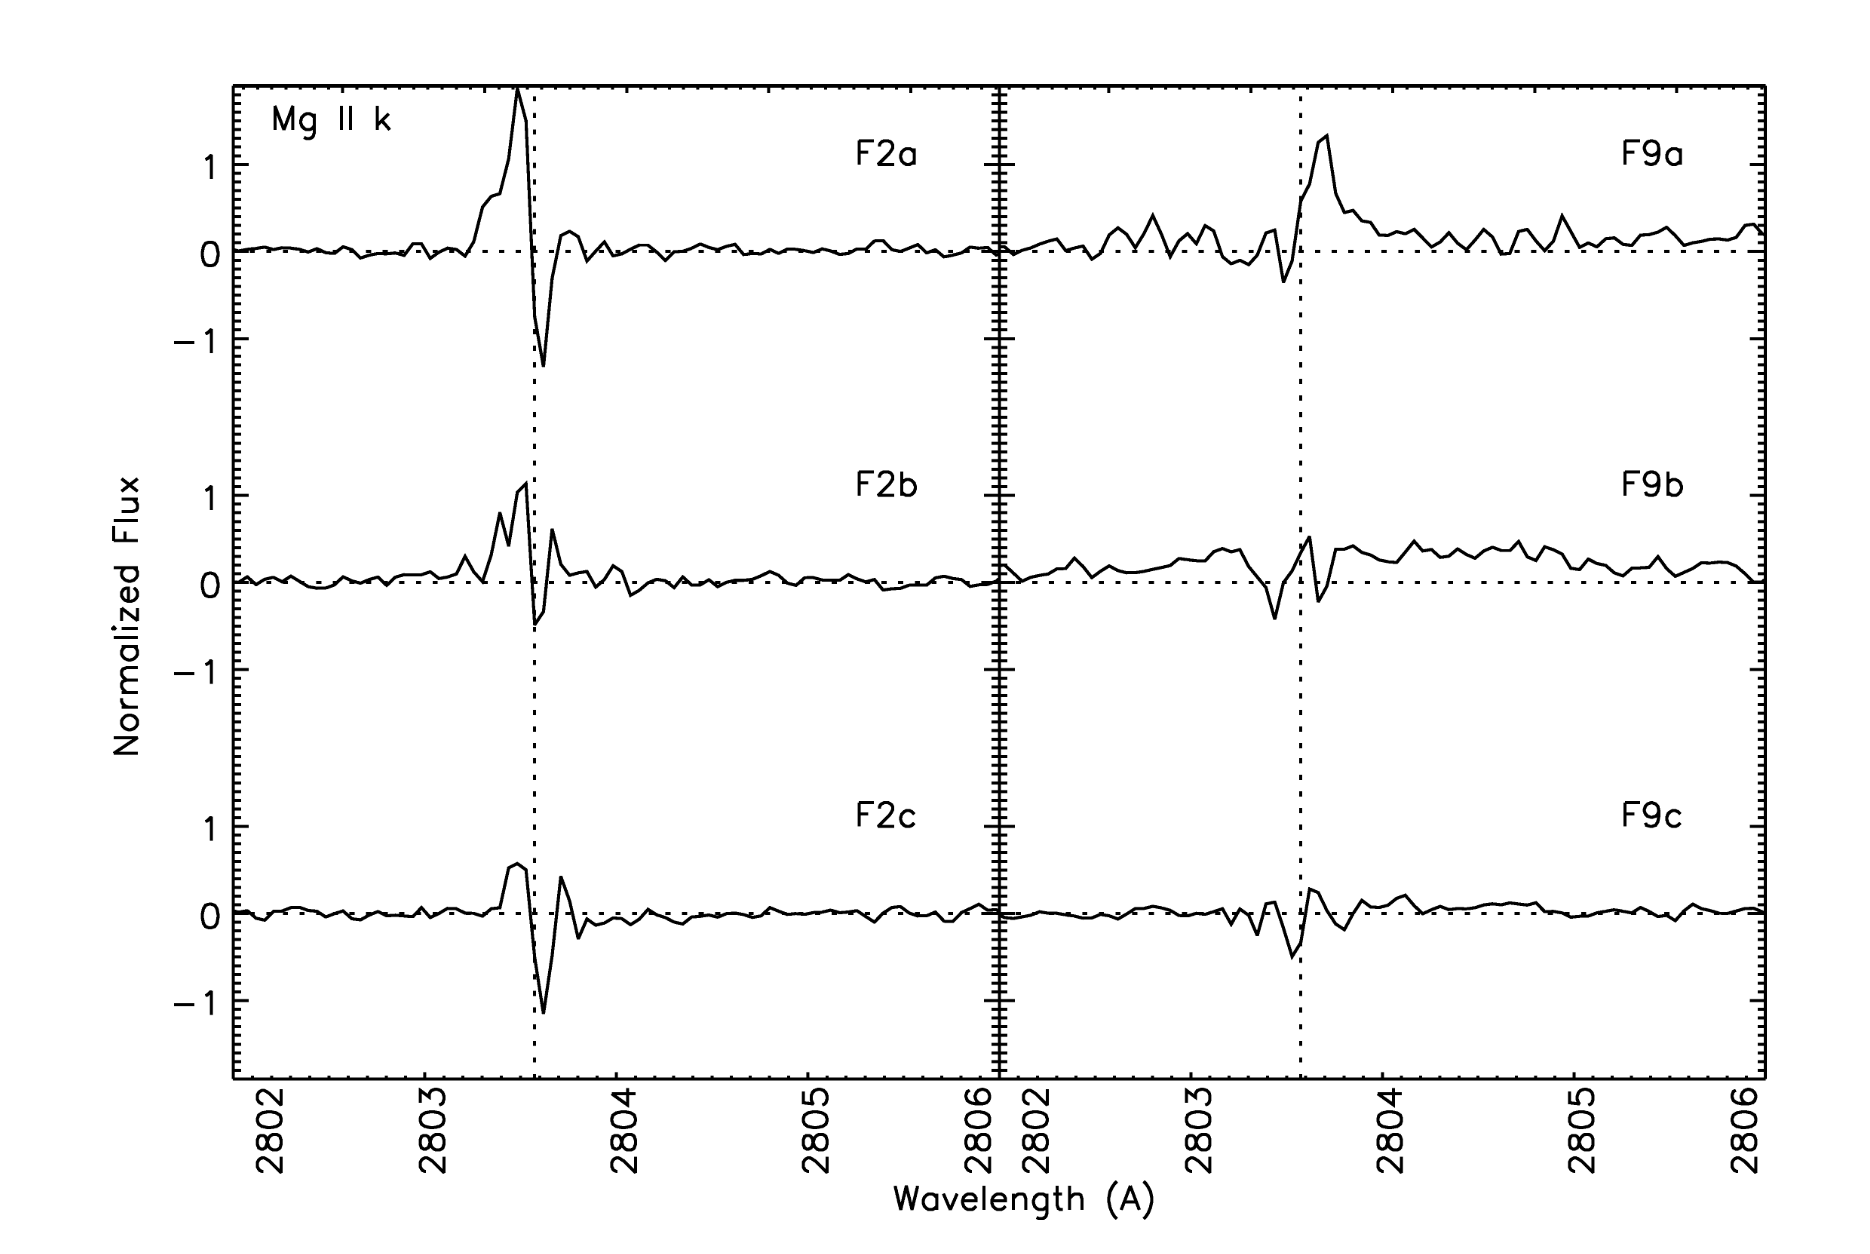
\includegraphics[width=0.5\textwidth]{figs/Hawley2007}
	\caption{两个M矮星上的大耀斑中观测到的Mg \textsc{ii} k线净轮廓。来源:\textcites{Hawley2007}}
	\label{fig:4.10}
\end{figure}

\begin{figure}
	\centering
	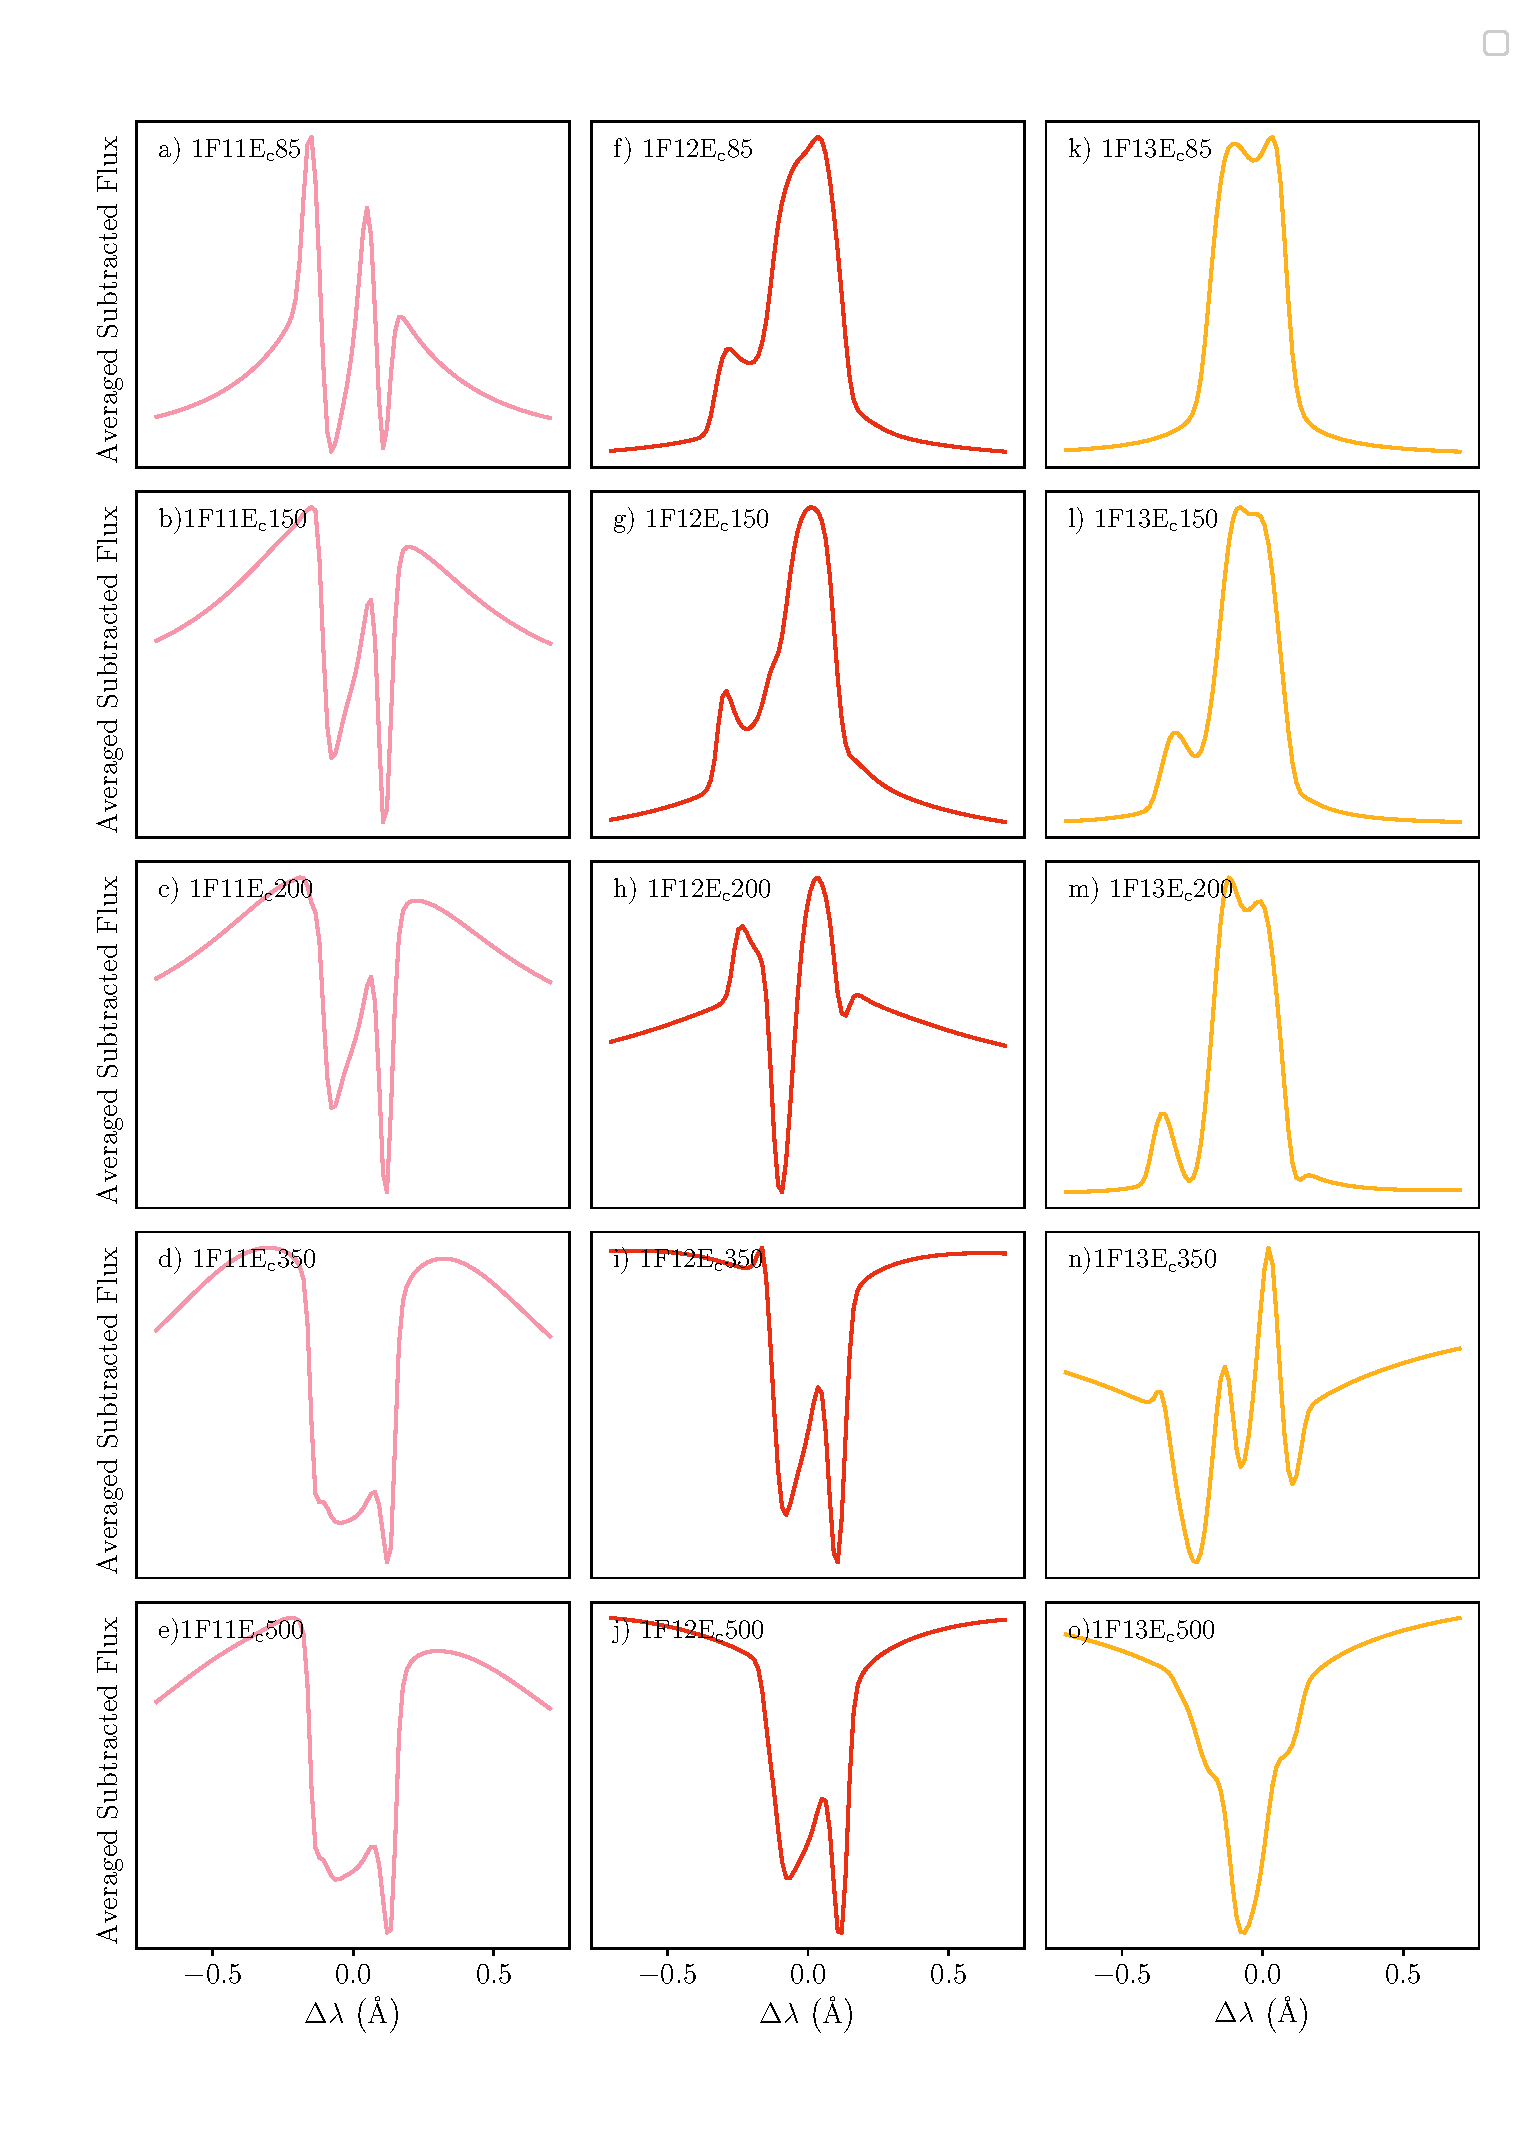
\includegraphics[width=\textwidth]{figs/dMe_MgIIh_spec_aver}
	\caption{Mg \textsc{ii} h线在不同电子束参数加热情况下对整个模拟过程取平均后的净辐射流量(已经减去初始宁静大气的辐射)。}
	\label{fig:4.11}
\end{figure}





% vim:ts=4:sw=4